
\documentclass{article}
%%%%%%%%%%%%%%%%%%%%%%%%%%%%%%%%%%%%%%%%%%%%%%%%%%%%%%%%%%%%%%%%%%%%%%%%%%%%%%%%%%%%%%%%%%%%%%%%%%%%%%%%%%%%%%%%%%%%%%%%%%%%%%%%%%%%%%%%%%%%%%%%%%%%%%%%%%%%%%%%%%%%%%%%%%%%%%%%%%%%%%%%%%%%%%%%%%%%%%%%%%%%%%%%%%%%%%%%%%%%%%%%%%%%%%%%%%%%%%%%%%%%%%%%%%%%
\usepackage{amsmath}
\usepackage{amssymb}
\usepackage{amsfonts}
\usepackage{graphicx}

\setcounter{MaxMatrixCols}{10}
%TCIDATA{OutputFilter=LATEX.DLL}
%TCIDATA{Version=5.50.0.2960}
%TCIDATA{<META NAME="SaveForMode" CONTENT="1">}
%TCIDATA{BibliographyScheme=Manual}
%TCIDATA{Created=Saturday, August 10, 2013 22:44:33}
%TCIDATA{LastRevised=Wednesday, January 13, 2016 18:15:13}
%TCIDATA{<META NAME="GraphicsSave" CONTENT="32">}
%TCIDATA{<META NAME="DocumentShell" CONTENT="Standard LaTeX\Blank - Standard LaTeX Article">}
%TCIDATA{CSTFile=40 LaTeX article.cst}

\newtheorem{theorem}{Theorem}
\newtheorem{acknowledgement}[theorem]{Acknowledgement}
\newtheorem{algorithm}[theorem]{Algorithm}
\newtheorem{axiom}[theorem]{Axiom}
\newtheorem{case}[theorem]{Case}
\newtheorem{claim}[theorem]{Claim}
\newtheorem{conclusion}[theorem]{Conclusion}
\newtheorem{condition}[theorem]{Condition}
\newtheorem{conjecture}[theorem]{Conjecture}
\newtheorem{corollary}[theorem]{Corollary}
\newtheorem{criterion}[theorem]{Criterion}
\newtheorem{definition}[theorem]{Definition}
\newtheorem{example}[theorem]{Example}
\newtheorem{exercise}[theorem]{Exercise}
\newtheorem{lemma}[theorem]{Lemma}
\newtheorem{notation}[theorem]{Notation}
\newtheorem{problem}[theorem]{Problem}
\newtheorem{proposition}[theorem]{Proposition}
\newtheorem{remark}[theorem]{Remark}
\newtheorem{solution}[theorem]{Solution}
\newtheorem{summary}[theorem]{Summary}
\newenvironment{proof}[1][Proof]{\noindent\textbf{#1.} }{\ \rule{0.5em}{0.5em}}
\setlength{\topmargin}{0cm}
\setlength{\textheight}{21.5cm}
\setlength{\textwidth}{16.5cm}
\setlength{\oddsidemargin}{0cm}
\renewcommand{\baselinestretch}{1}
% Macros for Scientific Word 2.5 documents saved with the LaTeX filter.
%Copyright (C) 1994-95 TCI Software Research, Inc.
\typeout{TCILATEX Macros for Scientific Word 2.5 <22 Dec 95>.}
\typeout{NOTICE:  This macro file is NOT proprietary and may be 
freely copied and distributed.}
%
\makeatletter
%
%%%%%%%%%%%%%%%%%%%%%%
% macros for time
\newcount\@hour\newcount\@minute\chardef\@x10\chardef\@xv60
\def\tcitime{
\def\@time{%
  \@minute\time\@hour\@minute\divide\@hour\@xv
  \ifnum\@hour<\@x 0\fi\the\@hour:%
  \multiply\@hour\@xv\advance\@minute-\@hour
  \ifnum\@minute<\@x 0\fi\the\@minute
  }}%

%%%%%%%%%%%%%%%%%%%%%%
% macro for hyperref
\@ifundefined{hyperref}{\def\hyperref#1#2#3#4{#2\ref{#4}#3}}{}

% macro for external program call
\@ifundefined{qExtProgCall}{\def\qExtProgCall#1#2#3#4#5#6{\relax}}{}
%%%%%%%%%%%%%%%%%%%%%%
%
% macros for graphics
%
\def\FILENAME#1{#1}%
%
\def\QCTOpt[#1]#2{%
  \def\QCTOptB{#1}
  \def\QCTOptA{#2}
}
\def\QCTNOpt#1{%
  \def\QCTOptA{#1}
  \let\QCTOptB\empty
}
\def\Qct{%
  \@ifnextchar[{%
    \QCTOpt}{\QCTNOpt}
}
\def\QCBOpt[#1]#2{%
  \def\QCBOptB{#1}
  \def\QCBOptA{#2}
}
\def\QCBNOpt#1{%
  \def\QCBOptA{#1}
  \let\QCBOptB\empty
}
\def\Qcb{%
  \@ifnextchar[{%
    \QCBOpt}{\QCBNOpt}
}
\def\PrepCapArgs{%
  \ifx\QCBOptA\empty
    \ifx\QCTOptA\empty
      {}%
    \else
      \ifx\QCTOptB\empty
        {\QCTOptA}%
      \else
        [\QCTOptB]{\QCTOptA}%
      \fi
    \fi
  \else
    \ifx\QCBOptA\empty
      {}%
    \else
      \ifx\QCBOptB\empty
        {\QCBOptA}%
      \else
        [\QCBOptB]{\QCBOptA}%
      \fi
    \fi
  \fi
}
\newcount\GRAPHICSTYPE
%\GRAPHICSTYPE 0 is for TurboTeX
%\GRAPHICSTYPE 1 is for DVIWindo (PostScript)
%%%(removed)%\GRAPHICSTYPE 2 is for psfig (PostScript)
\GRAPHICSTYPE=\z@
\def\GRAPHICSPS#1{%
 \ifcase\GRAPHICSTYPE%\GRAPHICSTYPE=0
   \special{ps: #1}%
 \or%\GRAPHICSTYPE=1
   \special{language "PS", include "#1"}%
%%%\or%\GRAPHICSTYPE=2
%%%  #1%
 \fi
}%
%
\def\GRAPHICSHP#1{\special{include #1}}%
%
% \graffile{ body }                                  %#1
%          { contentswidth (scalar)  }               %#2
%          { contentsheight (scalar) }               %#3
%          { vertical shift when in-line (scalar) }  %#4
\def\graffile#1#2#3#4{%
%%% \ifnum\GRAPHICSTYPE=\tw@
%%%  %Following if using psfig
%%%  \@ifundefined{psfig}{\input psfig.tex}{}%
%%%  \psfig{file=#1, height=#3, width=#2}%
%%% \else
  %Following for all others
  % JCS - added BOXTHEFRAME, see below
    \leavevmode
    \raise -#4 \BOXTHEFRAME{%
        \hbox to #2{\raise #3\hbox to #2{\null #1\hfil}}}%
}%
%
% A box for drafts
\def\draftbox#1#2#3#4{%
 \leavevmode\raise -#4 \hbox{%
  \frame{\rlap{\protect\tiny #1}\hbox to #2%
   {\vrule height#3 width\z@ depth\z@\hfil}%
  }%
 }%
}%
%
\newcount\draft
\draft=\z@
\let\nographics=\draft
\newif\ifwasdraft
\wasdraftfalse

%  \GRAPHIC{ body }                                  %#1
%          { draft name }                            %#2
%          { contentswidth (scalar)  }               %#3
%          { contentsheight (scalar) }               %#4
%          { vertical shift when in-line (scalar) }  %#5
\def\GRAPHIC#1#2#3#4#5{%
 \ifnum\draft=\@ne\draftbox{#2}{#3}{#4}{#5}%
  \else\graffile{#1}{#3}{#4}{#5}%
  \fi
 }%
%
\def\addtoLaTeXparams#1{%
    \edef\LaTeXparams{\LaTeXparams #1}}%
%
% JCS -  added a switch BoxFrame that can 
% be set by including X in the frame params.
% If set a box is drawn around the frame.

\newif\ifBoxFrame \BoxFramefalse
\newif\ifOverFrame \OverFramefalse
\newif\ifUnderFrame \UnderFramefalse

\def\BOXTHEFRAME#1{%
   \hbox{%
      \ifBoxFrame
         \frame{#1}%
      \else
         {#1}%
      \fi
   }%
}


\def\doFRAMEparams#1{\BoxFramefalse\OverFramefalse\UnderFramefalse\readFRAMEparams#1\end}%
\def\readFRAMEparams#1{%
 \ifx#1\end%
  \let\next=\relax
  \else
  \ifx#1i\dispkind=\z@\fi
  \ifx#1d\dispkind=\@ne\fi
  \ifx#1f\dispkind=\tw@\fi
  \ifx#1t\addtoLaTeXparams{t}\fi
  \ifx#1b\addtoLaTeXparams{b}\fi
  \ifx#1p\addtoLaTeXparams{p}\fi
  \ifx#1h\addtoLaTeXparams{h}\fi
  \ifx#1X\BoxFrametrue\fi
  \ifx#1O\OverFrametrue\fi
  \ifx#1U\UnderFrametrue\fi
  \ifx#1w
    \ifnum\draft=1\wasdrafttrue\else\wasdraftfalse\fi
    \draft=\@ne
  \fi
  \let\next=\readFRAMEparams
  \fi
 \next
 }%
%
%Macro for In-line graphics object
%   \IFRAME{ contentswidth (scalar)  }               %#1
%          { contentsheight (scalar) }               %#2
%          { vertical shift when in-line (scalar) }  %#3
%          { draft name }                            %#4
%          { body }                                  %#5
%          { caption}                                %#6


\def\IFRAME#1#2#3#4#5#6{%
      \bgroup
      \let\QCTOptA\empty
      \let\QCTOptB\empty
      \let\QCBOptA\empty
      \let\QCBOptB\empty
      #6%
      \parindent=0pt%
      \leftskip=0pt
      \rightskip=0pt
      \setbox0 = \hbox{\QCBOptA}%
      \@tempdima = #1\relax
      \ifOverFrame
          % Do this later
          \typeout{This is not implemented yet}%
          \show\HELP
      \else
         \ifdim\wd0>\@tempdima
            \advance\@tempdima by \@tempdima
            \ifdim\wd0 >\@tempdima
               \textwidth=\@tempdima
               \setbox1 =\vbox{%
                  \noindent\hbox to \@tempdima{\hfill\GRAPHIC{#5}{#4}{#1}{#2}{#3}\hfill}\\%
                  \noindent\hbox to \@tempdima{\parbox[b]{\@tempdima}{\QCBOptA}}%
               }%
               \wd1=\@tempdima
            \else
               \textwidth=\wd0
               \setbox1 =\vbox{%
                 \noindent\hbox to \wd0{\hfill\GRAPHIC{#5}{#4}{#1}{#2}{#3}\hfill}\\%
                 \noindent\hbox{\QCBOptA}%
               }%
               \wd1=\wd0
            \fi
         \else
            %\show\BBB
            \ifdim\wd0>0pt
              \hsize=\@tempdima
              \setbox1 =\vbox{%
                \unskip\GRAPHIC{#5}{#4}{#1}{#2}{0pt}%
                \break
                \unskip\hbox to \@tempdima{\hfill \QCBOptA\hfill}%
              }%
              \wd1=\@tempdima
           \else
              \hsize=\@tempdima
              \setbox1 =\vbox{%
                \unskip\GRAPHIC{#5}{#4}{#1}{#2}{0pt}%
              }%
              \wd1=\@tempdima
           \fi
         \fi
         \@tempdimb=\ht1
         \advance\@tempdimb by \dp1
         \advance\@tempdimb by -#2%
         \advance\@tempdimb by #3%
         \leavevmode
         \raise -\@tempdimb \hbox{\box1}%
      \fi
      \egroup%
}%
%
%Macro for Display graphics object
%   \DFRAME{ contentswidth (scalar)  }               %#1
%          { contentsheight (scalar) }               %#2
%          { draft label }                           %#3
%          { name }                                  %#4
%          { caption}                                %#5
\def\DFRAME#1#2#3#4#5{%
 \begin{center}
     \let\QCTOptA\empty
     \let\QCTOptB\empty
     \let\QCBOptA\empty
     \let\QCBOptB\empty
     \ifOverFrame 
        #5\QCTOptA\par
     \fi
     \GRAPHIC{#4}{#3}{#1}{#2}{\z@}
     \ifUnderFrame 
        \nobreak\par #5\QCBOptA
     \fi
 \end{center}%
 }%
%
%Macro for Floating graphic object
%   \FFRAME{ framedata f|i tbph x F|T }              %#1
%          { contentswidth (scalar)  }               %#2
%          { contentsheight (scalar) }               %#3
%          { caption }                               %#4
%          { label }                                 %#5
%          { draft name }                            %#6
%          { body }                                  %#7
\def\FFRAME#1#2#3#4#5#6#7{%
 \begin{figure}[#1]%
  \let\QCTOptA\empty
  \let\QCTOptB\empty
  \let\QCBOptA\empty
  \let\QCBOptB\empty
  \ifOverFrame
    #4
    \ifx\QCTOptA\empty
    \else
      \ifx\QCTOptB\empty
        \caption{\QCTOptA}%
      \else
        \caption[\QCTOptB]{\QCTOptA}%
      \fi
    \fi
    \ifUnderFrame\else
      \label{#5}%
    \fi
  \else
    \UnderFrametrue%
  \fi
  \begin{center}\GRAPHIC{#7}{#6}{#2}{#3}{\z@}\end{center}%
  \ifUnderFrame
    #4
    \ifx\QCBOptA\empty
      \caption{}%
    \else
      \ifx\QCBOptB\empty
        \caption{\QCBOptA}%
      \else
        \caption[\QCBOptB]{\QCBOptA}%
      \fi
    \fi
    \label{#5}%
  \fi
  \end{figure}%
 }%
%
%
%    \FRAME{ framedata f|i tbph x F|T }              %#1
%          { contentswidth (scalar)  }               %#2
%          { contentsheight (scalar) }               %#3
%          { vertical shift when in-line (scalar) }  %#4
%          { caption }                               %#5
%          { label }                                 %#6
%          { name }                                  %#7
%          { body }                                  %#8
%
%    framedata is a string which can contain the following
%    characters: idftbphxFT
%    Their meaning is as follows:
%             i, d or f : in-line, display, or floating
%             t,b,p,h   : LaTeX floating placement options
%             x         : fit contents box to contents
%             F or T    : Figure or Table. 
%                         Later this can expand
%                         to a more general float class.
%
%
\newcount\dispkind%

\def\makeactives{
  \catcode`\"=\active
  \catcode`\;=\active
  \catcode`\:=\active
  \catcode`\'=\active
  \catcode`\~=\active
}
\bgroup
   \makeactives
   \gdef\activesoff{%
      \def"{\string"}
      \def;{\string;}
      \def:{\string:}
      \def'{\string'}
      \def~{\string~}
      %\bbl@deactivate{"}%
      %\bbl@deactivate{;}%
      %\bbl@deactivate{:}%
      %\bbl@deactivate{'}%
    }
\egroup

\def\FRAME#1#2#3#4#5#6#7#8{%
 \bgroup
 \@ifundefined{bbl@deactivate}{}{\activesoff}
 \ifnum\draft=\@ne
   \wasdrafttrue
 \else
   \wasdraftfalse%
 \fi
 \def\LaTeXparams{}%
 \dispkind=\z@
 \def\LaTeXparams{}%
 \doFRAMEparams{#1}%
 \ifnum\dispkind=\z@\IFRAME{#2}{#3}{#4}{#7}{#8}{#5}\else
  \ifnum\dispkind=\@ne\DFRAME{#2}{#3}{#7}{#8}{#5}\else
   \ifnum\dispkind=\tw@
    \edef\@tempa{\noexpand\FFRAME{\LaTeXparams}}%
    \@tempa{#2}{#3}{#5}{#6}{#7}{#8}%
    \fi
   \fi
  \fi
  \ifwasdraft\draft=1\else\draft=0\fi{}%
  \egroup
 }%
%
% This macro added to let SW gobble a parameter that
% should not be passed on and expanded. 

\def\TEXUX#1{"texux"}

%
% Macros for text attributes:
%
\def\BF#1{{\bf {#1}}}%
\def\NEG#1{\leavevmode\hbox{\rlap{\thinspace/}{$#1$}}}%
%
%%%%%%%%%%%%%%%%%%%%%%%%%%%%%%%%%%%%%%%%%%%%%%%%%%%%%%%%%%%%%%%%%%%%%%%%
%
%
% macros for user - defined functions
\def\func#1{\mathop{\rm #1}}%
\def\limfunc#1{\mathop{\rm #1}}%

%
% miscellaneous 
%\long\def\QQQ#1#2{}%
\long\def\QQQ#1#2{%
     \long\expandafter\def\csname#1\endcsname{#2}}%
%\def\QTP#1{}% JCS - this was changed becuase style editor will define QTP
\@ifundefined{QTP}{\def\QTP#1{}}{}
\@ifundefined{QEXCLUDE}{\def\QEXCLUDE#1{}}{}
%\@ifundefined{Qcb}{\def\Qcb#1{#1}}{}
%\@ifundefined{Qct}{\def\Qct#1{#1}}{}
\@ifundefined{Qlb}{\def\Qlb#1{#1}}{}
\@ifundefined{Qlt}{\def\Qlt#1{#1}}{}
\def\QWE{}%
\long\def\QQA#1#2{}%
%\def\QTR#1#2{{\em #2}}% Always \em!!!
%\def\QTR#1#2{\mbox{\begin{#1}#2\end{#1}}}%cb%%%
\def\QTR#1#2{{\csname#1\endcsname #2}}%(gp) Is this the best?
\long\def\TeXButton#1#2{#2}%
\long\def\QSubDoc#1#2{#2}%
\def\EXPAND#1[#2]#3{}%
\def\NOEXPAND#1[#2]#3{}%
\def\PROTECTED{}%
\def\LaTeXparent#1{}%
\def\ChildStyles#1{}%
\def\ChildDefaults#1{}%
\def\QTagDef#1#2#3{}%
%
% Macros for style editor docs
\@ifundefined{StyleEditBeginDoc}{\def\StyleEditBeginDoc{\relax}}{}
%
% Macros for footnotes
\def\QQfnmark#1{\footnotemark}
\def\QQfntext#1#2{\addtocounter{footnote}{#1}\footnotetext{#2}}
%
% Macros for indexing.
\def\MAKEINDEX{\makeatletter\input gnuindex.sty\makeatother\makeindex}%	
\@ifundefined{INDEX}{\def\INDEX#1#2{}{}}{}%
\@ifundefined{SUBINDEX}{\def\SUBINDEX#1#2#3{}{}{}}{}%
\@ifundefined{initial}%  
   {\def\initial#1{\bigbreak{\raggedright\large\bf #1}\kern 2\p@\penalty3000}}%
   {}%
\@ifundefined{entry}{\def\entry#1#2{\item {#1}, #2}}{}%
\@ifundefined{primary}{\def\primary#1{\item {#1}}}{}%
\@ifundefined{secondary}{\def\secondary#1#2{\subitem {#1}, #2}}{}%
%
%
\@ifundefined{ZZZ}{}{\MAKEINDEX\makeatletter}%
%
% Attempts to avoid problems with other styles
\@ifundefined{abstract}{%
 \def\abstract{%
  \if@twocolumn
   \section*{Abstract (Not appropriate in this style!)}%
   \else \small 
   \begin{center}{\bf Abstract\vspace{-.5em}\vspace{\z@}}\end{center}%
   \quotation 
   \fi
  }%
 }{%
 }%
\@ifundefined{endabstract}{\def\endabstract
  {\if@twocolumn\else\endquotation\fi}}{}%
\@ifundefined{maketitle}{\def\maketitle#1{}}{}%
\@ifundefined{affiliation}{\def\affiliation#1{}}{}%
\@ifundefined{proof}{\def\proof{\noindent{\bfseries Proof. }}}{}%
\@ifundefined{endproof}{\def\endproof{\mbox{\ \rule{.1in}{.1in}}}}{}%
\@ifundefined{newfield}{\def\newfield#1#2{}}{}%
\@ifundefined{chapter}{\def\chapter#1{\par(Chapter head:)#1\par }%
 \newcount\c@chapter}{}%
\@ifundefined{part}{\def\part#1{\par(Part head:)#1\par }}{}%
\@ifundefined{section}{\def\section#1{\par(Section head:)#1\par }}{}%
\@ifundefined{subsection}{\def\subsection#1%
 {\par(Subsection head:)#1\par }}{}%
\@ifundefined{subsubsection}{\def\subsubsection#1%
 {\par(Subsubsection head:)#1\par }}{}%
\@ifundefined{paragraph}{\def\paragraph#1%
 {\par(Subsubsubsection head:)#1\par }}{}%
\@ifundefined{subparagraph}{\def\subparagraph#1%
 {\par(Subsubsubsubsection head:)#1\par }}{}%
%%%%%%%%%%%%%%%%%%%%%%%%%%%%%%%%%%%%%%%%%%%%%%%%%%%%%%%%%%%%%%%%%%%%%%%%
% These symbols are not recognized by LaTeX
\@ifundefined{therefore}{\def\therefore{}}{}%
\@ifundefined{backepsilon}{\def\backepsilon{}}{}%
\@ifundefined{yen}{\def\yen{\hbox{\rm\rlap=Y}}}{}%
\@ifundefined{registered}{%
   \def\registered{\relax\ifmmode{}\r@gistered
                    \else$\m@th\r@gistered$\fi}%
 \def\r@gistered{^{\ooalign
  {\hfil\raise.07ex\hbox{$\scriptstyle\rm\text{R}$}\hfil\crcr
  \mathhexbox20D}}}}{}%
\@ifundefined{Eth}{\def\Eth{}}{}%
\@ifundefined{eth}{\def\eth{}}{}%
\@ifundefined{Thorn}{\def\Thorn{}}{}%
\@ifundefined{thorn}{\def\thorn{}}{}%
% A macro to allow any symbol that requires math to appear in text
\def\TEXTsymbol#1{\mbox{$#1$}}%
\@ifundefined{degree}{\def\degree{{}^{\circ}}}{}%
%
% macros for T3TeX files
\newdimen\theight
\def\Column{%
 \vadjust{\setbox\z@=\hbox{\scriptsize\quad\quad tcol}%
  \theight=\ht\z@\advance\theight by \dp\z@\advance\theight by \lineskip
  \kern -\theight \vbox to \theight{%
   \rightline{\rlap{\box\z@}}%
   \vss
   }%
  }%
 }%
%
\def\qed{%
 \ifhmode\unskip\nobreak\fi\ifmmode\ifinner\else\hskip5\p@\fi\fi
 \hbox{\hskip5\p@\vrule width4\p@ height6\p@ depth1.5\p@\hskip\p@}%
 }%
%
\def\cents{\hbox{\rm\rlap/c}}%
\def\miss{\hbox{\vrule height2\p@ width 2\p@ depth\z@}}%
%\def\miss{\hbox{.}}%        %another possibility 
%
\def\vvert{\Vert}%           %always translated to \left| or \right|
%
\def\tcol#1{{\baselineskip=6\p@ \vcenter{#1}} \Column}  %
%
\def\dB{\hbox{{}}}%                 %dummy entry in column 
\def\mB#1{\hbox{$#1$}}%             %column entry
\def\nB#1{\hbox{#1}}%               %column entry (not math)
%
%\newcount\notenumber
%\def\clearnotenumber{\notenumber=0}
%\def\note{\global\advance\notenumber by 1
% \footnote{$^{\the\notenumber}$}}
%\def\note{\global\advance\notenumber by 1
\def\note{$^{\dag}}%
%
%

\def\newfmtname{LaTeX2e}
\def\chkcompat{%
   \if@compatibility
   \else
     \usepackage{latexsym}
   \fi
}

\ifx\fmtname\newfmtname
  \DeclareOldFontCommand{\rm}{\normalfont\rmfamily}{\mathrm}
  \DeclareOldFontCommand{\sf}{\normalfont\sffamily}{\mathsf}
  \DeclareOldFontCommand{\tt}{\normalfont\ttfamily}{\mathtt}
  \DeclareOldFontCommand{\bf}{\normalfont\bfseries}{\mathbf}
  \DeclareOldFontCommand{\it}{\normalfont\itshape}{\mathit}
  \DeclareOldFontCommand{\sl}{\normalfont\slshape}{\@nomath\sl}
  \DeclareOldFontCommand{\sc}{\normalfont\scshape}{\@nomath\sc}
  \chkcompat
\fi

%
% Greek bold macros
% Redefine all of the math symbols 
% which might be bolded	 - there are 
% probably others to add to this list

\def\alpha{\Greekmath 010B }%
\def\beta{\Greekmath 010C }%
\def\gamma{\Greekmath 010D }%
\def\delta{\Greekmath 010E }%
\def\epsilon{\Greekmath 010F }%
\def\zeta{\Greekmath 0110 }%
\def\eta{\Greekmath 0111 }%
\def\theta{\Greekmath 0112 }%
\def\iota{\Greekmath 0113 }%
\def\kappa{\Greekmath 0114 }%
\def\lambda{\Greekmath 0115 }%
\def\mu{\Greekmath 0116 }%
\def\nu{\Greekmath 0117 }%
\def\xi{\Greekmath 0118 }%
\def\pi{\Greekmath 0119 }%
\def\rho{\Greekmath 011A }%
\def\sigma{\Greekmath 011B }%
\def\tau{\Greekmath 011C }%
\def\upsilon{\Greekmath 011D }%
\def\phi{\Greekmath 011E }%
\def\chi{\Greekmath 011F }%
\def\psi{\Greekmath 0120 }%
\def\omega{\Greekmath 0121 }%
\def\varepsilon{\Greekmath 0122 }%
\def\vartheta{\Greekmath 0123 }%
\def\varpi{\Greekmath 0124 }%
\def\varrho{\Greekmath 0125 }%
\def\varsigma{\Greekmath 0126 }%
\def\varphi{\Greekmath 0127 }%

\def\nabla{\Greekmath 0272 }
\def\FindBoldGroup{%
   {\setbox0=\hbox{$\mathbf{x\global\edef\theboldgroup{\the\mathgroup}}$}}%
}

\def\Greekmath#1#2#3#4{%
    \if@compatibility
        \ifnum\mathgroup=\symbold
           \mathchoice{\mbox{\boldmath$\displaystyle\mathchar"#1#2#3#4$}}%
                      {\mbox{\boldmath$\textstyle\mathchar"#1#2#3#4$}}%
                      {\mbox{\boldmath$\scriptstyle\mathchar"#1#2#3#4$}}%
                      {\mbox{\boldmath$\scriptscriptstyle\mathchar"#1#2#3#4$}}%
        \else
           \mathchar"#1#2#3#4% 
        \fi 
    \else 
        \FindBoldGroup
        \ifnum\mathgroup=\theboldgroup % For 2e
           \mathchoice{\mbox{\boldmath$\displaystyle\mathchar"#1#2#3#4$}}%
                      {\mbox{\boldmath$\textstyle\mathchar"#1#2#3#4$}}%
                      {\mbox{\boldmath$\scriptstyle\mathchar"#1#2#3#4$}}%
                      {\mbox{\boldmath$\scriptscriptstyle\mathchar"#1#2#3#4$}}%
        \else
           \mathchar"#1#2#3#4% 
        \fi     	    
	  \fi}

\newif\ifGreekBold  \GreekBoldfalse
\let\SAVEPBF=\pbf
\def\pbf{\GreekBoldtrue\SAVEPBF}%
%

\@ifundefined{theorem}{\newtheorem{theorem}{Theorem}}{}
\@ifundefined{lemma}{\newtheorem{lemma}[theorem]{Lemma}}{}
\@ifundefined{corollary}{\newtheorem{corollary}[theorem]{Corollary}}{}
\@ifundefined{conjecture}{\newtheorem{conjecture}[theorem]{Conjecture}}{}
\@ifundefined{proposition}{\newtheorem{proposition}[theorem]{Proposition}}{}
\@ifundefined{axiom}{\newtheorem{axiom}{Axiom}}{}
\@ifundefined{remark}{\newtheorem{remark}{Remark}}{}
\@ifundefined{example}{\newtheorem{example}{Example}}{}
\@ifundefined{exercise}{\newtheorem{exercise}{Exercise}}{}
\@ifundefined{definition}{\newtheorem{definition}{Definition}}{}


\@ifundefined{mathletters}{%
  %\def\theequation{\arabic{equation}}
  \newcounter{equationnumber}  
  \def\mathletters{%
     \addtocounter{equation}{1}
     \edef\@currentlabel{\theequation}%
     \setcounter{equationnumber}{\c@equation}
     \setcounter{equation}{0}%
     \edef\theequation{\@currentlabel\noexpand\alph{equation}}%
  }
  \def\endmathletters{%
     \setcounter{equation}{\value{equationnumber}}%
  }
}{}

%Logos
\@ifundefined{BibTeX}{%
    \def\BibTeX{{\rm B\kern-.05em{\sc i\kern-.025em b}\kern-.08em
                 T\kern-.1667em\lower.7ex\hbox{E}\kern-.125emX}}}{}%
\@ifundefined{AmS}%
    {\def\AmS{{\protect\usefont{OMS}{cmsy}{m}{n}%
                A\kern-.1667em\lower.5ex\hbox{M}\kern-.125emS}}}{}%
\@ifundefined{AmSTeX}{\def\AmSTeX{\protect\AmS-\protect\TeX\@}}{}%
%

%%%%%%%%%%%%%%%%%%%%%%%%%%%%%%%%%%%%%%%%%%%%%%%%%%%%%%%%%%%%%%%%%%%%%%%
% NOTE: The rest of this file is read only if amstex has not been
% loaded.  This section is used to define amstex constructs in the
% event they have not been defined.
%
%
\ifx\ds@amstex\relax
   \message{amstex already loaded}\makeatother\endinput% 2.09 compatability
\else
   \@ifpackageloaded{amstex}%
      {\message{amstex already loaded}\makeatother\endinput}
      {}
   \@ifpackageloaded{amsgen}%
      {\message{amsgen already loaded}\makeatother\endinput}
      {}
\fi
%%%%%%%%%%%%%%%%%%%%%%%%%%%%%%%%%%%%%%%%%%%%%%%%%%%%%%%%%%%%%%%%%%%%%%%%
%%
%
%
%  Macros to define some AMS LaTeX constructs when 
%  AMS LaTeX has not been loaded
% 
% These macros are copied from the AMS-TeX package for doing
% multiple integrals.
%
\let\DOTSI\relax
\def\RIfM@{\relax\ifmmode}%
\def\FN@{\futurelet\next}%
\newcount\intno@
\def\iint{\DOTSI\intno@\tw@\FN@\ints@}%
\def\iiint{\DOTSI\intno@\thr@@\FN@\ints@}%
\def\iiiint{\DOTSI\intno@4 \FN@\ints@}%
\def\idotsint{\DOTSI\intno@\z@\FN@\ints@}%
\def\ints@{\findlimits@\ints@@}%
\newif\iflimtoken@
\newif\iflimits@
\def\findlimits@{\limtoken@true\ifx\next\limits\limits@true
 \else\ifx\next\nolimits\limits@false\else
 \limtoken@false\ifx\ilimits@\nolimits\limits@false\else
 \ifinner\limits@false\else\limits@true\fi\fi\fi\fi}%
\def\multint@{\int\ifnum\intno@=\z@\intdots@                          %1
 \else\intkern@\fi                                                    %2
 \ifnum\intno@>\tw@\int\intkern@\fi                                   %3
 \ifnum\intno@>\thr@@\int\intkern@\fi                                 %4
 \int}%                                                               %5
\def\multintlimits@{\intop\ifnum\intno@=\z@\intdots@\else\intkern@\fi
 \ifnum\intno@>\tw@\intop\intkern@\fi
 \ifnum\intno@>\thr@@\intop\intkern@\fi\intop}%
\def\intic@{%
    \mathchoice{\hskip.5em}{\hskip.4em}{\hskip.4em}{\hskip.4em}}%
\def\negintic@{\mathchoice
 {\hskip-.5em}{\hskip-.4em}{\hskip-.4em}{\hskip-.4em}}%
\def\ints@@{\iflimtoken@                                              %1
 \def\ints@@@{\iflimits@\negintic@
   \mathop{\intic@\multintlimits@}\limits                             %2
  \else\multint@\nolimits\fi                                          %3
  \eat@}%                                                             %4
 \else                                                                %5
 \def\ints@@@{\iflimits@\negintic@
  \mathop{\intic@\multintlimits@}\limits\else
  \multint@\nolimits\fi}\fi\ints@@@}%
\def\intkern@{\mathchoice{\!\!\!}{\!\!}{\!\!}{\!\!}}%
\def\plaincdots@{\mathinner{\cdotp\cdotp\cdotp}}%
\def\intdots@{\mathchoice{\plaincdots@}%
 {{\cdotp}\mkern1.5mu{\cdotp}\mkern1.5mu{\cdotp}}%
 {{\cdotp}\mkern1mu{\cdotp}\mkern1mu{\cdotp}}%
 {{\cdotp}\mkern1mu{\cdotp}\mkern1mu{\cdotp}}}%
%
%
%  These macros are for doing the AMS \text{} construct
%
\def\RIfM@{\relax\protect\ifmmode}
\def\text{\RIfM@\expandafter\text@\else\expandafter\mbox\fi}
\let\nfss@text\text
\def\text@#1{\mathchoice
   {\textdef@\displaystyle\f@size{#1}}%
   {\textdef@\textstyle\tf@size{\firstchoice@false #1}}%
   {\textdef@\textstyle\sf@size{\firstchoice@false #1}}%
   {\textdef@\textstyle \ssf@size{\firstchoice@false #1}}%
   \glb@settings}

\def\textdef@#1#2#3{\hbox{{%
                    \everymath{#1}%
                    \let\f@size#2\selectfont
                    #3}}}
\newif\iffirstchoice@
\firstchoice@true
%
%    Old Scheme for \text
%
%\def\rmfam{\z@}%
%\newif\iffirstchoice@
%\firstchoice@true
%\def\textfonti{\the\textfont\@ne}%
%\def\textfontii{\the\textfont\tw@}%
%\def\text{\RIfM@\expandafter\text@\else\expandafter\text@@\fi}%
%\def\text@@#1{\leavevmode\hbox{#1}}%
%\def\text@#1{\mathchoice
% {\hbox{\everymath{\displaystyle}\def\textfonti{\the\textfont\@ne}%
%  \def\textfontii{\the\textfont\tw@}\textdef@@ T#1}}%
% {\hbox{\firstchoice@false
%  \everymath{\textstyle}\def\textfonti{\the\textfont\@ne}%
%  \def\textfontii{\the\textfont\tw@}\textdef@@ T#1}}%
% {\hbox{\firstchoice@false
%  \everymath{\scriptstyle}\def\textfonti{\the\scriptfont\@ne}%
%  \def\textfontii{\the\scriptfont\tw@}\textdef@@ S\rm#1}}%
% {\hbox{\firstchoice@false
%  \everymath{\scriptscriptstyle}\def\textfonti
%  {\the\scriptscriptfont\@ne}%
%  \def\textfontii{\the\scriptscriptfont\tw@}\textdef@@ s\rm#1}}}%
%\def\textdef@@#1{\textdef@#1\rm\textdef@#1\bf\textdef@#1\sl
%    \textdef@#1\it}%
%\def\DN@{\def\next@}%
%\def\eat@#1{}%
%\def\textdef@#1#2{%
% \DN@{\csname\expandafter\eat@\string#2fam\endcsname}%
% \if S#1\edef#2{\the\scriptfont\next@\relax}%
% \else\if s#1\edef#2{\the\scriptscriptfont\next@\relax}%
% \else\edef#2{\the\textfont\next@\relax}\fi\fi}%
%
%
%These are the AMS constructs for multiline limits.
%
\def\Let@{\relax\iffalse{\fi\let\\=\cr\iffalse}\fi}%
\def\vspace@{\def\vspace##1{\crcr\noalign{\vskip##1\relax}}}%
\def\multilimits@{\bgroup\vspace@\Let@
 \baselineskip\fontdimen10 \scriptfont\tw@
 \advance\baselineskip\fontdimen12 \scriptfont\tw@
 \lineskip\thr@@\fontdimen8 \scriptfont\thr@@
 \lineskiplimit\lineskip
 \vbox\bgroup\ialign\bgroup\hfil$\m@th\scriptstyle{##}$\hfil\crcr}%
\def\Sb{_\multilimits@}%
\def\endSb{\crcr\egroup\egroup\egroup}%
\def\Sp{^\multilimits@}%
\let\endSp\endSb
%
%
%These are AMS constructs for horizontal arrows
%
\newdimen\ex@
\ex@.2326ex
\def\rightarrowfill@#1{$#1\m@th\mathord-\mkern-6mu\cleaders
 \hbox{$#1\mkern-2mu\mathord-\mkern-2mu$}\hfill
 \mkern-6mu\mathord\rightarrow$}%
\def\leftarrowfill@#1{$#1\m@th\mathord\leftarrow\mkern-6mu\cleaders
 \hbox{$#1\mkern-2mu\mathord-\mkern-2mu$}\hfill\mkern-6mu\mathord-$}%
\def\leftrightarrowfill@#1{$#1\m@th\mathord\leftarrow
\mkern-6mu\cleaders
 \hbox{$#1\mkern-2mu\mathord-\mkern-2mu$}\hfill
 \mkern-6mu\mathord\rightarrow$}%
\def\overrightarrow{\mathpalette\overrightarrow@}%
\def\overrightarrow@#1#2{\vbox{\ialign{##\crcr\rightarrowfill@#1\crcr
 \noalign{\kern-\ex@\nointerlineskip}$\m@th\hfil#1#2\hfil$\crcr}}}%
\let\overarrow\overrightarrow
\def\overleftarrow{\mathpalette\overleftarrow@}%
\def\overleftarrow@#1#2{\vbox{\ialign{##\crcr\leftarrowfill@#1\crcr
 \noalign{\kern-\ex@\nointerlineskip}$\m@th\hfil#1#2\hfil$\crcr}}}%
\def\overleftrightarrow{\mathpalette\overleftrightarrow@}%
\def\overleftrightarrow@#1#2{\vbox{\ialign{##\crcr
   \leftrightarrowfill@#1\crcr
 \noalign{\kern-\ex@\nointerlineskip}$\m@th\hfil#1#2\hfil$\crcr}}}%
\def\underrightarrow{\mathpalette\underrightarrow@}%
\def\underrightarrow@#1#2{\vtop{\ialign{##\crcr$\m@th\hfil#1#2\hfil
  $\crcr\noalign{\nointerlineskip}\rightarrowfill@#1\crcr}}}%
\let\underarrow\underrightarrow
\def\underleftarrow{\mathpalette\underleftarrow@}%
\def\underleftarrow@#1#2{\vtop{\ialign{##\crcr$\m@th\hfil#1#2\hfil
  $\crcr\noalign{\nointerlineskip}\leftarrowfill@#1\crcr}}}%
\def\underleftrightarrow{\mathpalette\underleftrightarrow@}%
\def\underleftrightarrow@#1#2{\vtop{\ialign{##\crcr$\m@th
  \hfil#1#2\hfil$\crcr
 \noalign{\nointerlineskip}\leftrightarrowfill@#1\crcr}}}%
%%%%%%%%%%%%%%%%%%%%%

% 94.0815 by Jon:

\def\qopnamewl@#1{\mathop{\operator@font#1}\nlimits@}
\let\nlimits@\displaylimits
\def\setboxz@h{\setbox\z@\hbox}


\def\varlim@#1#2{\mathop{\vtop{\ialign{##\crcr
 \hfil$#1\m@th\operator@font lim$\hfil\crcr
 \noalign{\nointerlineskip}#2#1\crcr
 \noalign{\nointerlineskip\kern-\ex@}\crcr}}}}

 \def\rightarrowfill@#1{\m@th\setboxz@h{$#1-$}\ht\z@\z@
  $#1\copy\z@\mkern-6mu\cleaders
  \hbox{$#1\mkern-2mu\box\z@\mkern-2mu$}\hfill
  \mkern-6mu\mathord\rightarrow$}
\def\leftarrowfill@#1{\m@th\setboxz@h{$#1-$}\ht\z@\z@
  $#1\mathord\leftarrow\mkern-6mu\cleaders
  \hbox{$#1\mkern-2mu\copy\z@\mkern-2mu$}\hfill
  \mkern-6mu\box\z@$}


\def\projlim{\qopnamewl@{proj\,lim}}
\def\injlim{\qopnamewl@{inj\,lim}}
\def\varinjlim{\mathpalette\varlim@\rightarrowfill@}
\def\varprojlim{\mathpalette\varlim@\leftarrowfill@}
\def\varliminf{\mathpalette\varliminf@{}}
\def\varliminf@#1{\mathop{\underline{\vrule\@depth.2\ex@\@width\z@
   \hbox{$#1\m@th\operator@font lim$}}}}
\def\varlimsup{\mathpalette\varlimsup@{}}
\def\varlimsup@#1{\mathop{\overline
  {\hbox{$#1\m@th\operator@font lim$}}}}

%
%%%%%%%%%%%%%%%%%%%%%%%%%%%%%%%%%%%%%%%%%%%%%%%%%%%%%%%%%%%%%%%%%%%%%
%
\def\tfrac#1#2{{\textstyle {#1 \over #2}}}%
\def\dfrac#1#2{{\displaystyle {#1 \over #2}}}%
\def\binom#1#2{{#1 \choose #2}}%
\def\tbinom#1#2{{\textstyle {#1 \choose #2}}}%
\def\dbinom#1#2{{\displaystyle {#1 \choose #2}}}%
\def\QATOP#1#2{{#1 \atop #2}}%
\def\QTATOP#1#2{{\textstyle {#1 \atop #2}}}%
\def\QDATOP#1#2{{\displaystyle {#1 \atop #2}}}%
\def\QABOVE#1#2#3{{#2 \above#1 #3}}%
\def\QTABOVE#1#2#3{{\textstyle {#2 \above#1 #3}}}%
\def\QDABOVE#1#2#3{{\displaystyle {#2 \above#1 #3}}}%
\def\QOVERD#1#2#3#4{{#3 \overwithdelims#1#2 #4}}%
\def\QTOVERD#1#2#3#4{{\textstyle {#3 \overwithdelims#1#2 #4}}}%
\def\QDOVERD#1#2#3#4{{\displaystyle {#3 \overwithdelims#1#2 #4}}}%
\def\QATOPD#1#2#3#4{{#3 \atopwithdelims#1#2 #4}}%
\def\QTATOPD#1#2#3#4{{\textstyle {#3 \atopwithdelims#1#2 #4}}}%
\def\QDATOPD#1#2#3#4{{\displaystyle {#3 \atopwithdelims#1#2 #4}}}%
\def\QABOVED#1#2#3#4#5{{#4 \abovewithdelims#1#2#3 #5}}%
\def\QTABOVED#1#2#3#4#5{{\textstyle 
   {#4 \abovewithdelims#1#2#3 #5}}}%
\def\QDABOVED#1#2#3#4#5{{\displaystyle 
   {#4 \abovewithdelims#1#2#3 #5}}}%
%
% Macros for text size operators:

%JCS - added braces and \mathop around \displaystyle\int, etc.
%
\def\tint{\mathop{\textstyle \int}}%
\def\tiint{\mathop{\textstyle \iint }}%
\def\tiiint{\mathop{\textstyle \iiint }}%
\def\tiiiint{\mathop{\textstyle \iiiint }}%
\def\tidotsint{\mathop{\textstyle \idotsint }}%
\def\toint{\mathop{\textstyle \oint}}%
\def\tsum{\mathop{\textstyle \sum }}%
\def\tprod{\mathop{\textstyle \prod }}%
\def\tbigcap{\mathop{\textstyle \bigcap }}%
\def\tbigwedge{\mathop{\textstyle \bigwedge }}%
\def\tbigoplus{\mathop{\textstyle \bigoplus }}%
\def\tbigodot{\mathop{\textstyle \bigodot }}%
\def\tbigsqcup{\mathop{\textstyle \bigsqcup }}%
\def\tcoprod{\mathop{\textstyle \coprod }}%
\def\tbigcup{\mathop{\textstyle \bigcup }}%
\def\tbigvee{\mathop{\textstyle \bigvee }}%
\def\tbigotimes{\mathop{\textstyle \bigotimes }}%
\def\tbiguplus{\mathop{\textstyle \biguplus }}%
%
%
%Macros for display size operators:
%

\def\dint{\mathop{\displaystyle \int}}%
\def\diint{\mathop{\displaystyle \iint }}%
\def\diiint{\mathop{\displaystyle \iiint }}%
\def\diiiint{\mathop{\displaystyle \iiiint }}%
\def\didotsint{\mathop{\displaystyle \idotsint }}%
\def\doint{\mathop{\displaystyle \oint}}%
\def\dsum{\mathop{\displaystyle \sum }}%
\def\dprod{\mathop{\displaystyle \prod }}%
\def\dbigcap{\mathop{\displaystyle \bigcap }}%
\def\dbigwedge{\mathop{\displaystyle \bigwedge }}%
\def\dbigoplus{\mathop{\displaystyle \bigoplus }}%
\def\dbigodot{\mathop{\displaystyle \bigodot }}%
\def\dbigsqcup{\mathop{\displaystyle \bigsqcup }}%
\def\dcoprod{\mathop{\displaystyle \coprod }}%
\def\dbigcup{\mathop{\displaystyle \bigcup }}%
\def\dbigvee{\mathop{\displaystyle \bigvee }}%
\def\dbigotimes{\mathop{\displaystyle \bigotimes }}%
\def\dbiguplus{\mathop{\displaystyle \biguplus }}%
%
%Companion to stackrel
\def\stackunder#1#2{\mathrel{\mathop{#2}\limits_{#1}}}%
%
%
% These are AMS environments that will be defined to
% be verbatims if amstex has not actually been 
% loaded
%
%
\begingroup \catcode `|=0 \catcode `[= 1
\catcode`]=2 \catcode `\{=12 \catcode `\}=12
\catcode`\\=12 
|gdef|@alignverbatim#1\end{align}[#1|end[align]]
|gdef|@salignverbatim#1\end{align*}[#1|end[align*]]

|gdef|@alignatverbatim#1\end{alignat}[#1|end[alignat]]
|gdef|@salignatverbatim#1\end{alignat*}[#1|end[alignat*]]

|gdef|@xalignatverbatim#1\end{xalignat}[#1|end[xalignat]]
|gdef|@sxalignatverbatim#1\end{xalignat*}[#1|end[xalignat*]]

|gdef|@gatherverbatim#1\end{gather}[#1|end[gather]]
|gdef|@sgatherverbatim#1\end{gather*}[#1|end[gather*]]

|gdef|@gatherverbatim#1\end{gather}[#1|end[gather]]
|gdef|@sgatherverbatim#1\end{gather*}[#1|end[gather*]]


|gdef|@multilineverbatim#1\end{multiline}[#1|end[multiline]]
|gdef|@smultilineverbatim#1\end{multiline*}[#1|end[multiline*]]

|gdef|@arraxverbatim#1\end{arrax}[#1|end[arrax]]
|gdef|@sarraxverbatim#1\end{arrax*}[#1|end[arrax*]]

|gdef|@tabulaxverbatim#1\end{tabulax}[#1|end[tabulax]]
|gdef|@stabulaxverbatim#1\end{tabulax*}[#1|end[tabulax*]]


|endgroup
  

  
\def\align{\@verbatim \frenchspacing\@vobeyspaces \@alignverbatim
You are using the "align" environment in a style in which it is not defined.}
\let\endalign=\endtrivlist
 
\@namedef{align*}{\@verbatim\@salignverbatim
You are using the "align*" environment in a style in which it is not defined.}
\expandafter\let\csname endalign*\endcsname =\endtrivlist




\def\alignat{\@verbatim \frenchspacing\@vobeyspaces \@alignatverbatim
You are using the "alignat" environment in a style in which it is not defined.}
\let\endalignat=\endtrivlist
 
\@namedef{alignat*}{\@verbatim\@salignatverbatim
You are using the "alignat*" environment in a style in which it is not defined.}
\expandafter\let\csname endalignat*\endcsname =\endtrivlist




\def\xalignat{\@verbatim \frenchspacing\@vobeyspaces \@xalignatverbatim
You are using the "xalignat" environment in a style in which it is not defined.}
\let\endxalignat=\endtrivlist
 
\@namedef{xalignat*}{\@verbatim\@sxalignatverbatim
You are using the "xalignat*" environment in a style in which it is not defined.}
\expandafter\let\csname endxalignat*\endcsname =\endtrivlist




\def\gather{\@verbatim \frenchspacing\@vobeyspaces \@gatherverbatim
You are using the "gather" environment in a style in which it is not defined.}
\let\endgather=\endtrivlist
 
\@namedef{gather*}{\@verbatim\@sgatherverbatim
You are using the "gather*" environment in a style in which it is not defined.}
\expandafter\let\csname endgather*\endcsname =\endtrivlist


\def\multiline{\@verbatim \frenchspacing\@vobeyspaces \@multilineverbatim
You are using the "multiline" environment in a style in which it is not defined.}
\let\endmultiline=\endtrivlist
 
\@namedef{multiline*}{\@verbatim\@smultilineverbatim
You are using the "multiline*" environment in a style in which it is not defined.}
\expandafter\let\csname endmultiline*\endcsname =\endtrivlist


\def\arrax{\@verbatim \frenchspacing\@vobeyspaces \@arraxverbatim
You are using a type of "array" construct that is only allowed in AmS-LaTeX.}
\let\endarrax=\endtrivlist

\def\tabulax{\@verbatim \frenchspacing\@vobeyspaces \@tabulaxverbatim
You are using a type of "tabular" construct that is only allowed in AmS-LaTeX.}
\let\endtabulax=\endtrivlist

 
\@namedef{arrax*}{\@verbatim\@sarraxverbatim
You are using a type of "array*" construct that is only allowed in AmS-LaTeX.}
\expandafter\let\csname endarrax*\endcsname =\endtrivlist

\@namedef{tabulax*}{\@verbatim\@stabulaxverbatim
You are using a type of "tabular*" construct that is only allowed in AmS-LaTeX.}
\expandafter\let\csname endtabulax*\endcsname =\endtrivlist

% macro to simulate ams tag construct


% This macro is a fix to eqnarray
\def\@@eqncr{\let\@tempa\relax
    \ifcase\@eqcnt \def\@tempa{& & &}\or \def\@tempa{& &}%
      \else \def\@tempa{&}\fi
     \@tempa
     \if@eqnsw
        \iftag@
           \@taggnum
        \else
           \@eqnnum\stepcounter{equation}%
        \fi
     \fi
     \global\tag@false
     \global\@eqnswtrue
     \global\@eqcnt\z@\cr}


% This macro is a fix to the equation environment
 \def\endequation{%
     \ifmmode\ifinner % FLEQN hack
      \iftag@
        \addtocounter{equation}{-1} % undo the increment made in the begin part
        $\hfil
           \displaywidth\linewidth\@taggnum\egroup \endtrivlist
        \global\tag@false
        \global\@ignoretrue   
      \else
        $\hfil
           \displaywidth\linewidth\@eqnnum\egroup \endtrivlist
        \global\tag@false
        \global\@ignoretrue 
      \fi
     \else   
      \iftag@
        \addtocounter{equation}{-1} % undo the increment made in the begin part
        \eqno \hbox{\@taggnum}
        \global\tag@false%
        $$\global\@ignoretrue
      \else
        \eqno \hbox{\@eqnnum}% $$ BRACE MATCHING HACK
        $$\global\@ignoretrue
      \fi
     \fi\fi
 } 

 \newif\iftag@ \tag@false
 
 \def\tag{\@ifnextchar*{\@tagstar}{\@tag}}
 \def\@tag#1{%
     \global\tag@true
     \global\def\@taggnum{(#1)}}
 \def\@tagstar*#1{%
     \global\tag@true
     \global\def\@taggnum{#1}%  
}

% Do not add anything to the end of this file.  
% The last section of the file is loaded only if 
% amstex has not been.



\makeatother
\endinput

\begin{document}

\title{A No-arbitrage Model of Liquidity in Financial Markets involving
Brownian Sheets\thanks{%
With the collaboration of Thanh Hoang and Jennifer Thompson.}}
\author{Henry Schellhorn and Ran Zhao\thanks{%
Claremont Graduate University}}
\date{\today }
\maketitle

\begin{abstract}
We consider a dynamic market model where buyers and sellers submit limit
orders. If at a given moment in time, the buyer is unable to complete his
entire order due to the shortage of sell orders at the required limit price,
the unmatched part of the order is recorded in the order book. Subsequently
these buy unmatched orders may be matched with new incoming sell orders. The
resulting demand curve constitutes the sole input to our model. The clearing
price is then mechanically calculated using the market clearing condition.
We assume a continuous model for the demand curve. We show that generically
there exists an equivalent martingale measure for the clearing price if the
driving noise is a Brownian sheet, while there may not be if the driving
noise is multidimensional Brownian motion.

Another contribution of this paper is to prove that, if there exists an
equivalent martingale measure for the clearing price, then, under some mild
assumptions, there is no arbitrage. We use the Ito-Wentzell formula to
obtain both results. We also characterize the dynamics of the demand curve
and of the clearing price in the equivalent martingale measure. We find that
the volatility of the clearing price is inversely proportional to the sum of
buy and sell order flow density (evaluated at the clearing price), which
confirms the intuition that volatility is inversely proportional to volume.
We also demonstrate that our approach is implementable. We use real order
book data and simulate option prices under a particularly simple
parameterization of our model.

The no-arbitrage conditions we obtain are applicable to a wide class of
models, in the same way that the Heath-Jarrow-Morton conditions apply to a
wide class of interest rate models.
\end{abstract}

\section{Introduction}

Most liquidity models in mathematical finance abstract the trading mechanism
from the characterization of prices in the resulting market. Our viewpoint
is here fundamentally different. In our model, equilibrium prices of assets
are completely determined by the order flow, which is viewed as an exogenous
process. We model a market of assets without specialist where every trader
submits limit orders, that is, for a buy order, the buyer specifies the
maximum price, or buy limit price, that he/she is willing to pay, and, for a
sell order, the seller specifies the minimum price, or sell limit price, at
which he/she is willing to sell \footnote{%
There is no loss of generality in that statement. A buy market order can be
specified in our model as a buy limit order with limit price equal to
infinity. Since we model assets with only positive prices, a sell market
order can be specified in our model as a sell limit order with a limit price
equal to zero.}.

If at a given moment in time, the buyer is unable to complete his entire
order due to the shortage of sell orders at the required limit price, the
unmatched part of the order is recorded in the order book.A symmetric
outcome exists in the case of incoming sell orders. Subsequently these buy
unmatched orders may be matched with new incoming sell orders.We note that
many electronic exchanges, such as NYSE\ ARCA, operate like this.
Time-priority is used to break indeterminacies of a match between an
incoming buyer at limit price superior to the ask price, i.e., the lowest
limit price in the sell order book. As a result, the equilibrium of \textit{%
clearing price} process is always defined.

Since the matching mechanism does not add any information to the economy,
all information about asset prices is included in the order flow. Whether
public exchanges should or should not reveal in real-time the data contained
in the order book is an important issue, which continues to preoccupy the
financial markets community [WW02]. Our theoretical framework accommodates
either viewpoint, but our empirical application is better tailored to the
viewpoint that order books are public information. The current blossoming of
high-frequency trading activity [Eng00],[BLT06], [Hau08], [SM08], [BRZ]
seems to confirm our viewpoint that traders are (i) interested in
understanding order book information, and (ii) trade on that information.

We do not address in this paper the issue of differential information
further. The market microstructure literature (such as [Kyl85], and all
following models) considers various models of trading involving uninformed
traders, called noise traders, and one, or several informed traders. One of
the key results of the Kyle model is that, given the information available
to noise traders, the resulting price process is a martingale in the
appropriate measure, whereas it may not be for the informed traders. As a
consequence we do not believe that abstracting issues of differential
information is limiting. The order books reflect all the public information.
Public information corresponds to the filtration under which the clearing
price needs to have an equivalent martingale measure, in order to avoid
arbitrage. Obviously, the clearing price may not be a martingale in the
aforementioned measure if the filtration is enlarged to include private
information.

There are roughly two different class of models in the liquidity literature.
The first class of models ([Jar92, [Jar94], [PS98a], [PS98b], [Fre98],
[SW00], [BB04], [RS10]) considers the action of a large trader who can
manipulate the prices in the market. There are mainly two different types of
strategies a large trader can employ to that effect. The first one is to
corner the market, and then squeeze the shorts.\ The second one is to
"front-run one's own trades". While some exchanges have rules to curtail the
cornering of the market, front-running seems more difficult to ban from an
exchange. It is known in discrete-time trading, that, if there is no
possibility of arbitrage in periods where the large investor does not trade,
then there is no market manipulation strategy.

The second class of models ([CJP04], [CR07], [CST10],[GS11]) abstracts the
issues of market manipulation away, and considers all traders as
price-takers. In particular, [CJP04] introduced an exogenous residual supply
curve against which an investor trades. The investor trades market orders,
and his/her order is matched instantaneously. As a consequence of the
instantaneity, it is plausible for [CJP04] to assume the "price effect of an
order is limited to the very moment when the order is placed in the market"
(dixit [BB04]), so that that the residual supply curve at a future time is
statistically independent from the order just matched. For us however, this
assumption is not convenient, since it does not explain how prices can
incorporate information from the arrival of new orders.

Our model belongs to the first class of models. We define our demand curve
as quantity as a function of price, unlike most other authors, who define it
as price as a function of quantity. While both definitions contain the same
information, we found it necessary to have a representation of the demand
curve as quantity as a function of price in order to characterize the
clearing price $\pi (t)$. We may thus as well start from there in order to
avoid technical problems due to inverting the demand curve. In this sense,
we extend the [BB04] paper, where the clearing price is not characterized,
in the direction followed by [CJP04], where the clearing price is
characterized.

We proceed in two steps to define our model. In the first step, we consider
a market with atomistic traders and a large trader. By assumption, the net
demand curve of the atomistic traders is\ a smooth semimartingale family. We
argue that, if the large trader is rational, his net demand curve should
also be a smooth semimartingale family. Since the sum of two smooth
semimartingale families is also a smooth semimartingale family, the market
net demand curve is also a smooth semimartingale family when the market
consists of both atomistic traders and one rational large trader in the
market. We do not want however to limit the applicability of our paper to
such a model. Thus, in a second step, we start by assuming that the market
net demand curve is a smooth semimartingale family. Alternate theoretical
constructions may justify this assumption. For practitioners, only an
empirical verification of this assumption is necessary for them to use the
market model.

In our model all the information is contained in a Brownian sheet, which
drives the dynamics of the market net demand curve. The advantage of using a
Brownian sheet is that we have the same cardinality of independent sources
of noise (namely, the cardinality of a real interval) as the cardinality of
the set of exogenous stochastic processes, namely net demand at each limit
price. Because of that reason, there exists (generically)\ an equivalent
martingale measure for the clearing price, while there would not be any if
the driving noise was Brownian motion, or multidimensional Brownian motion%
\footnote{%
This is analogous to traditional market models in mathematical finance.
Equality of the number of risk factors and number of securities is
(generically)\ necessary to obtain an equivalent martingale measure. In our
liquidity model, each point on the net demand curve is analogous to an
individual security.}. We use the Ito-Wentzell formula to obtain this
result. The second main result in our article is to prove that, if there is
an equivalent martingale measure $\mathbb{Q}$ for the clearing price $\pi
(t) $, then, under some mild assumptions there is no arbitrage, as in [BB04].

We do not claim that it is indispensable to use a Brownian sheet to model an
arbitrage-free limit order market. In an ingenious construction [KR09] use
Carmona-Nualart [CT90] stochastic integration to weaken the assumptions in
the [BB04] necessary to avoid arbitrage. They show for instance that a
simple Bachelier model is arbitrage-free. Unfortunately, the result of
inverting the net demand curve in the Bachelier model has singularities
which prevented us from characterizing the clearing price as well as using
the Ito-Wentzell formula.

We characterize the dynamics of the demand curve and of the clearing price
in the measure $\mathbb{Q}$. We find that the volatility of the clearing
price is inversely proportional to the sum of buy and sell order flow
density (evaluated at the clearing price), which confirms the intuition that
volatility is inversely proportional to volume.

We also demonstrate that our approach is implementable. Although we do not
prove a second fundamental theorem of asset pricing, we naively use a
special parameterization of our model to price options. As in the early days
of the Heath-Jarrow-Morton methodology, we use only historical estimation
(in our case, of the order book)\ to fit our model and solve for the market
price of risk. We expect that, should this paper meet with interest around
practitioners, market-implied implementations will see the day.
Unsurprisingly, we obtain a smile curve for implied volatility. We note that
this particular feature is not a very strong sign of the adequacy of our
approach to model asset prices, as most models that came after Black-Scholes
[BS73]\ result in a smile curve for implied volatility. Although limited,
our results are however encouraging. They show that a fairly demanding
theoretical model can be easily implemented.

The structure of the paper is as follows. In section 2, we introduce our
model and show our main results: existence of an equivalent martingale
measure for the clearing price $\pi $ and absence of arbitrage. In section 3
we analyze the Bachelier model, and show how it would be difficult to make
it fit our framework. In section 4, we describe our data set and the
methodology we used to extract it. Finally, section 5 shows our
implementation, namely a simulation of option prices under the risk-neutral
measure.

\section{Preliminaries}

\subsection{The Market Mechanism}

\noindent A buy\ limit order specifies how many shares a trader wants to
buy, and at what maximum price he is willing to buy them. We call this price
the (buy) \textit{limit price}. A buy\ limit order specifies how many shares
a trader wants to buy, and at what maximum price he is willing to buy them.
We call this price the (sell)\ \textit{limit price}. Both buy and sell limit
prices are denoted by $p$, and should not be confused with the clearing
price, which is denoted by $\pi (t)$. The unmatched buy and sell orders are
stored in order books, until they are either cancelled or matched with an
incoming order. An incoming order is matched with the order in the opposite
side of the market which has the best price. The clearing price of the
transaction is equal to the limit price of the order in the book, and not of
the incoming order. Partial execution is allowed, and, ties are resolved by
time-priority. We give herafter an example of the matching mechanism in
discrete time, i.e., at most one order arrives at time $t\in \{0,1,2,..\}.$

\textbf{Example}

Suppose that the clearing price at time $0$ is any price $\pi (0)\in \lbrack
100,120]$. After clearing, that is, when $0<t<1$ we suppose that the order
books contain the following orders

\begin{equation*}
\begin{tabular}{|l|l|}
\hline
\multicolumn{2}{|l|}{Buy Order Book} \\
Price & Quantity \\ \hline\hline
100 & 10 \\ \hline
\end{tabular}%
\text{ \ \ \ \ \ }%
\begin{tabular}{|l|l|}
\hline
\multicolumn{2}{|l|}{Sell Order Book} \\
Price & Quantity \\ \hline\hline
120 & 10 \\ \hline
130 & 10 \\ \hline
\end{tabular}%
\end{equation*}

At time $t=1$ a buy order arrives with a limit price of \$125, and a
quantity of 15. The exchange matches it with the best sell order, i.e., the
one with a sell limit price of \$120. However, execution is only partial,
and the remainder of the buy order is placed in the order book at the limit
price of \$120, resulting in the following order books:

\begin{equation*}
\begin{tabular}{|l|l|}
\hline
\multicolumn{2}{|l|}{Buy Order Book} \\
Price & Quantity \\ \hline\hline
100 & 10 \\ \hline
125 & 5 \\ \hline
\end{tabular}%
\text{ \ \ \ \ \ }%
\begin{tabular}{|l|l|}
\hline
\multicolumn{2}{|l|}{Sell Order Book} \\
Price & Quantity \\ \hline\hline
130 & 10 \\ \hline
\end{tabular}%
\end{equation*}

The clearing price at time 1 is equal to the limit price of the sell order,
i.e.:

\begin{equation*}
\pi (1)=120
\end{equation*}

$\blacksquare $

This example illustrates several properties of limit order markets. First,
the clearing price is always defined, and can assume any positive value%
\footnote{%
We do not consider markets for swaps, where the price can be negative.}.

Second, it is not inconceivable that an incoming order "crosses" the order
book, i.e., for the case of a buy order, that its limit price is higher than
the best sell order limit price (i.e, the best ask), since the buyer does
not lose a cent. Crossing the book is indeed advantageous for two reasons:
first, it allows for faster execution. In our example, had the buyer
submitted an order at price \$130 he would have bought the complete quantity
of shares (15)\ that he desired, rather than waiting an indeterminate amount
of time until enough sell arrives arrive until enough sell arrives arrive at
his limit price. Second, suppose that several buy orders are submitted at
the same time. In case the demand exceeds the supply at the best ask, the
buy orders with the highest limit price are executed first. Our own data
analysis (see section 4) shows that few orders cross the Arca book. This is
consistent with the theory of optimal order book placement suggested by Rosu
[Ros09].

\bigskip

\subsection{The Brownian Sheet}

We now move to continuous-time. Be aware that we do not prove convergence of
a discrete-time model to our continuous-time model. We take the latter as a
given, plausible model of the market. We start with a filtered probability
space $(\Omega ,\mathcal{F},\{\mathcal{F}_{t}\},\mathbb{P})$ satisfying the
usual conditions. All the uncertainty is described by a one-dimensional
Brownian sheet $W(t,s)$ which generates $\{\mathcal{F}_{t}\}$.There are
several approaches to construct a Brownian sheet, or, more generally
stochastic partial differential equations. According to Mueller [Mue09] "One
can use either Walsh's [Wal86] approach [..], the Hilbert space approach of
Da Prato and Zabczyk [DPZ92], or Krylov's [Kry06] $L_{p}$ theory". [DPZ92]
and [Mue09] note that the approach is at least as general as the [Wal86]
approach. We use the Hilbert space approach as exposed in [CT06].

\bigskip

We wish to make sense of the Brownian sheet and of its stochastic integral:

\begin{equation}
I_{t}=\int_{u=0}^{t}\int_{s=0}^{S}b(s,u)W(ds,du)  \label{continuous}
\end{equation}%
\bigskip

where $W$ is a Brownian sheet and, for each $s\in \lbrack 0,S]$ the $%
\mathcal{F}_{t}-$adapted stochastic process $b(s,t)$ satisfies:%
\begin{equation*}
\int_{s=0}^{S}b^{2}(s,t)ds=1
\end{equation*}

We first define $W_{t}$ as a random variable on the space $E\equiv
L^{2}[0,S] $ such that $W=\{W_{t}$;$t\in \lbrack 0,T]\}$ is an $E-$ valued
Wiener process. If we let $\{e_{n}^{\ast };n\geq 1\}$ be a complete
orthonormal basis of the dual $H^{\ast }$of the reproducing kernel Hilbert
space $H$ of $E$ and define:

\begin{equation*}
w_{n}(t)=e_{n}^{\ast }(W_{t})
\end{equation*}

we have:

\begin{equation}
W_{t}=\sum_{n=1}^{\infty }w_{n}(t)e_{n}  \label{nonconvergent}
\end{equation}

where $w_{n}$ are independent $\mathbb{R}$-valued standard Wiener processes.
While the series (\ref{nonconvergent})\ is not convergent in $E$ in $l^{2}$,
we can define the following integral (see [DPZ92] p. 100)

\begin{equation*}
W(s,t)=\sum_{n=1}^{\infty }w_{n}(t)\int_{0}^{s}e_{n}(\alpha )d\alpha \text{
\ \ }s\in \lbrack 0,S]
\end{equation*}

which is our Brownian sheet. We now define a family of operators $B_{t}$:$%
E\rightarrow \mathbb{R}$ for $t\in \lbrack 0,T]$ by the formula:

\begin{equation*}
B_{t}f=\int_{s=0}^{S}b(s,t)f(s)ds
\end{equation*}

Since $B$ is a Hilbert-Schmidt operator, we can also write this expression
as:

\begin{equation*}
B_{t}f=\sum_{n=1}^{\infty }b^{n}(t)e_{n}^{\ast }(f)
\end{equation*}

for some real-valued $\mathcal{F}_{t}-$adapted stochastic processes $b^{n}$
satisfying:

\begin{equation*}
b^{n}(t)=e_{n}^{\ast }(b(.,t))
\end{equation*}

Thus, we have the definition:

\begin{equation}
I_{t}=\int_{u=0}^{t}\sum_{n=1}^{\infty }b^{n}(u)dw_{n}(u)  \label{Forkrylov}
\end{equation}

We will use expression (\ref{continuous})\ for most of the text since it
will be convenient to see $b(s,u)W(ds,du)$ as being indexed by the continuum
$s\in \lbrack 0,S]$. However expression (\ref{Forkrylov})\ is\ an equally
valid expression and will allow us to use directly the Ito-Wentzell formula
as developed in [Kry09]. Finally, we note that in Walsh's approach the
definitions (\ref{nonconvergent}) and (\ref{Forkrylov}) do not involve
infinite series, but for our purpose the approaches are equivalent. For a
rigorous comparison of the two approaches, we refer the reader to [DQ11].

\bigskip

\subsection{A Market with Atomistic Traders and a Large Trader}

\textbf{Assumption 1 }(Assumption A1 in\textbf{\ }[Ja92]).\ The market is
frictionless.

\bigskip

\textbf{Assumption 2 }Buy and sell limit prices can assume any real value
between $0$ and $S$. Orders can be submitted to the market at any time $t\in
\mathbb{R}^{+}$.

\bigskip

\textbf{Notation} Buy and sell limit prices are usually denoted by $p$. The
market clearing price is denoted by $\pi $.

\bigskip

\textbf{Definitions: }the net demand curve $Q_{A}$ of the atomistic traders
is a function $[0,S]\times \mathbb{R}^{+}\times \Omega \mathbb{\rightarrow R}
$ which value $Q_{A}(p,t,\omega )$\ is equal to the difference between the
quantity of shares \textbf{submitted} for purchase (at price lower than or
equal to $p$) and the quantity of shares \textbf{submitted} for sale (at
price larger than or equal to $p$) between time.zero and time $t$ by
atomistic traders. The same definition holds for the the net demand curve $%
Q_{L}$ of the large trader

\bigskip

\textbf{Remark: }We do not define precisely what we mean by atomistic
traders. We view them as a continuum of traders. Each of them submits an
infinitesimally small orders at a price $p$, such that there is no
concentration of orders at any particular price, as we formulate more
clearly below, in contradistinction with the large trader.

\bigskip

\textbf{Assumption 3 }For each\textbf{\ }$t$ the net demand curve\textbf{\ }$%
Q_{A}$ is twice-differentiable in the first argument.

\bigskip

\textbf{Remark:} For a fixed price $p$ the total quantity of shares
submitted for purchase \ does not need to be increasing in time, as some
orders may be cancelled. However, it has to be a positive value.

\bigskip

\textbf{Assumption 4: }The net demand curve $Q_{A}$ is strictly decreasing
in its first argument, for all $p$ except $p=0$ and $p=S$.

\bigskip

\textbf{Remark} The fact that net demand curves are decreasing is an
immediate consequence of our market mechanism (see above), and the fact that
order quantities are by definition positive. Indeed, the number of shares of
available buy orders is decreasing in price, while the number of shares is
of available sell orders is increasing. The net demand, being the difference
of buy and sell orders, is a decreasing function of price. Assumption 4 is
similar to assumption A3 in [Ja92] or assumption 2 in [BB04].

\bigskip

\textbf{Assumption 5:}\ W suppose that the $\mathbb{R}$-valued $\mathcal{F}%
_{t}$-adapted processes coefficients $\mu _{Q_{A}}(p,.)$, $\sigma
_{Q_{A}}(p,.)$ and $b_{Q_{A}}(p,s,.)$, when evaluated at any time $t\in
\lbrack 0,T]$, belong to $L^{2}(\mathbb{P})$. The net demand curve of the
atomistic traders $Q_{A}$ satisfies:

\begin{eqnarray}
dQ_{A}(p,t,\omega ) &=&\mu _{Q_{A}}(p,t,\omega )dt+\sigma
_{Q_{A}}(p,t,\omega )\int_{s=0}^{S}b_{Q_{A}}(p,s,t,\omega )W(ds,dt,\omega )%
\text{ \ \ \ }0\leq p\leq S  \label{GenMod1} \\
Q_{A}(p,0) &=&Q_{A,0}(p)>0\text{ \ \ \ \ \ \ \ \ }0\leq p\leq S
\label{GenMod2} \\
\int_{s=0}^{S}b_{Q_{A}}^{2}(p,s,t,\omega ) &=&1\text{ \ \ \ \ \ \ \ \ }0\leq
p\leq S  \label{GenMod3}
\end{eqnarray}

\textbf{Remark:}\ We do not provide more specific assumptions on the
coefficients $\mu _{Q_{A}}$,$\sigma _{Q_{A}}$,$b_{Q_{A}}$ as we will define
later a more specific model which will satisfy all our assumptions,
including remark **. For the moment, we note that, by theorem 4.12 in
[DPZ92], each $Q_{A}(p,t.,.)$ is a $\mathcal{F}_{t}$-adapted
square-integrable semimartingale.

\bigskip

\textbf{Definition} the market net demand curve $Q$ is defined by:

\begin{equation}
Q=Q_{A}+Q_{L}  \label{defofQ}
\end{equation}

\textbf{Definition }The clearing price $\pi (t)$ is a $\mathcal{F}_{t}-$
adapted stochastic process which satisfies:

\begin{equation}
Q(\pi (t),t)=0  \label{pi}
\end{equation}

when there is a solution to (\ref{pi}), or is otherwise defined by
continuation, i.e., $\pi (t)$ is equal to the value of $\pi $ at the latest
time $s<t$ for which there was a solution to $Q(\pi (s),s)=0$. We show in
the next section a particular model where there is always a solution to (\ref%
{pi}).

\bigskip

\textbf{Definition:\ }The position of the large trader is denoted by $\theta
(t)$.

\bigskip

\textbf{Remark: }The position of the trader changes with the clearing price,
as well as with the net demand curve:

\begin{eqnarray}
d\theta (t) &=&d(Q_{L}(\pi (t),t))  \label{theta_1} \\
&=&-d(Q_{A}(\pi (t),t))  \label{theta_2}
\end{eqnarray}

\textbf{Definition: }Suppose that $\theta (t)$ is equal to a constant $%
\vartheta $. The price $P_{A}(\vartheta ,t,\omega )$ available on the market
when the large trader position is $\vartheta $ is defined for each $t$ by

\begin{equation*}
Q_{A}(P_{A}(\vartheta ,t,\omega ),t,\omega )=\vartheta \text{ \ \ }\vartheta
\in \lbrack Q_{A}(\infty ,t,\omega ),Q_{A}(0,t,\omega )]
\end{equation*}

and otherwise by continuation.

\textbf{Definition:} As in [KR09] we denote by $S_{A}(\theta ,t)$ the price
available on the market when the large trader follows a time-varying
strategy $\theta (t)$. In other terms:

\begin{equation*}
S_{A}(\theta ,t)=P_{A}(\theta (t),t)
\end{equation*}

\textbf{Remark: }The clearing price satisfies:

\begin{equation*}
\pi (t)=\int_{0}^{t}S_{A}(\theta ,ds)
\end{equation*}

\textbf{Definition }[BB04]\textbf{\ }The asymptotic liquidation proceeeds of
the large trader, denoted by $L$ is equal to:\
\begin{equation*}
L(\vartheta ,t)=\int_{0}^{\vartheta }P_{A}(x,t)dx
\end{equation*}

\textbf{Definition }define\textbf{\ }$\beta ^{\theta }$\bigskip

\textbf{Definition} The real wealth process achieved by a self-financing
trading strategy $\theta $ is given by

\begin{equation*}
V^{\theta }(t)=\beta ^{\theta }(t)+L(\theta (t),t)
\end{equation*}

\textbf{Fact:}\ (lemma 3.2 in [BB04]) Provided that the $L(\theta )$ is a
smooth family of semimartingales (in the sense of [BB04]), for any
self-financing semimartingale strategy $\theta $, the dynamics of the real
wealth process $V^{\theta }$ are given by:

\begin{equation}
V^{\theta }(t)-V^{\theta }(0_{-})=\int_{0}^{t}L(\theta (u_{-}),du)-\frac{1}{2%
}\int_{0}^{t}P^{\prime }(\theta (u_{-}),u)d[\theta ,\theta
]_{s}^{c}-\sum_{0\leq u\leq t}\int_{\theta (u_{-})}^{\theta (u)}\{P(\theta
(u),u)-P(x,u)\}dx  \label{lemma32BB04}
\end{equation}

\textbf{Definition} An arbitrage (strategy) is a self-financing trading
strategy $\theta $ such that $V^{\theta }(0_{-})=0$ and:

\begin{eqnarray*}
P(V^{\theta }(t) &>&0)>0 \\
P(V^{\theta }(t) &\geq &0)\geq 0
\end{eqnarray*}

\textbf{Lemma 1: } Let:

\begin{eqnarray*}
\mu _{P}(x,t) &=&-\frac{\mu _{Q_{A}}(P_{A}(x,t),t)+\frac{1}{2}\frac{\partial
^{2}Q_{A}}{\partial p^{2}}(P_{A}(x,t),t)\sigma _{P}^{2}(x,t)+\frac{\partial
\sigma _{Q_{A}}}{\partial p}(P_{A}(x,t),t)\sigma _{P}(t)}{\frac{\partial
Q_{A}}{\partial p}(P_{A}(x,t),t)} \\
\sigma _{P}(x,t) &=&\frac{\sigma _{Q_{A}}(P_{A}(x,t),t)}{\frac{\partial Q_{A}%
}{\partial p}(P_{A}(x,t),t)} \\
b_{P}(x,s,t) &=&-b_{Q_{A}}(P_{A}(x,t),s,t)
\end{eqnarray*}

Then the family $P_{A}(x)$ is a smooth family of semimartingales (in the
sense of definition 2.2 in [BB04]), and satisfies:

\begin{equation}
dP_{A}(x,t)=\mu _{P}(x,t)dt+\sigma
_{P}(x,t)\int\limits_{0}^{S}b_{P}(x,s,t)W(ds,dt)  \label{equforP}
\end{equation}%
\bigskip

\textbf{Proof of lemma:}

By definition:

\begin{equation}
Q_{A}(P(x,t),t)=x  \label{ItoWE}
\end{equation}

We suppose that (\ref{equforP})\ holds and apply the Ito-Wentzell formula
(see e.g., Krylov (2009))\ to both sides of (\ref{ItoWE}):

\begin{eqnarray*}
\mu _{Q_{A}}(P(x,t),t)+\frac{\partial Q_{A}}{\partial p}(P(x,t),t)\mu
_{P}(x,t)+\frac{1}{2}\frac{\partial ^{2}Q_{A}}{\partial p^{2}}%
(P(x,t),t)\sigma _{P}^{2}(x,t)+\frac{\partial \sigma _{Q_{A}}}{\partial p}%
(P(x,t),t)\sigma _{P}(x,t) &=&0 \\
\sigma _{Q_{A}}(P(x,t),t)b_{Q_{A}}(P(x,t),s,t)+\frac{\partial Q_{A}}{%
\partial p}(P(x,t),t)\sigma _{P}(x,t)b_{P}(x,s,t) &=&0
\end{eqnarray*}

Since, by assumption $\frac{\partial Q_{A}}{\partial p}<0$, the lemma
follows.

\bigskip

\textbf{Lemma 2 }If the large trader is rational \footnote{%
In the sense that he prefers more to less.} the net demand curve $Q_{L}$ and
the clearing price $\pi $ are continuous in $t$.

\bigskip

\textbf{Proof }\ The family of semimartingales $L(\vartheta )$ is smooth. We
skip the proof of this fact since it is identical (modulo replacing $Q_{A}$
by $Q$) to the proof that $L_{2}(\vartheta )$ is smooth, which figures in
the proof of theorem 1. Lemma 1 shows then that $P_{A}(x,t)$ is
well-defined, and thus the dynamics of the wealth process $V^{\theta }$ are
given by (\ref{lemma32BB04}). The latter equation shows that only tame
strategies for $\theta $ are rational, that is, $[\theta ,\theta ]^{c}=0$,
and $\theta $ is continuous. By (\ref{theta_1})

\begin{eqnarray*}
0 &=&\theta (t_{+})-\theta (t) \\
&=&-Q_{A}(\pi (t_{+}),t_{+})+Q_{A}(\pi (t),t) \\
&=&-Q_{A}(\pi (t_{+}),t_{+})+Q_{A}(\pi (t_{+}),t) \\
&&-Q_{A}(\pi (t_{+}),t)+Q_{A}(\pi (t),t)
\end{eqnarray*}

Since $Q_{A}$ is continuous

\begin{equation*}
Q_{A}(\pi (t_{+}),t_{+})-Q_{A}(\pi (t_{+}),t)=0
\end{equation*}

Thus

\begin{equation*}
Q_{A}(\pi (t_{+}),t)-Q_{A}(\pi (t),t)=0
\end{equation*}

Since $Q_{A}$ is strictly decreasing $\pi $ is continuous. Using (\ref%
{theta_1}):

\begin{eqnarray*}
0 &=&\theta (t_{+})-\theta (t) \\
&=&Q_{L}(\pi (t_{+}),t_{+})-Q_{L}(\pi (t),t) \\
&=&Q_{L}(\pi (t_{+}),t_{+})-Q_{L}(\pi (t_{+}),t) \\
&&+Q_{L}(\pi (t_{+}),t)-Q_{L}(\pi (t),t)
\end{eqnarray*}

Since $\pi $ is continuous$:$

\begin{equation*}
0=Q_{L}(\pi (t_{+}),t_{+})-Q_{L}(\pi (t_{+}),t)
\end{equation*}

Thus $Q_{L}$ is continuous in time. $\blacksquare $

\bigskip

\textbf{Lemma 3: }If the large trader is rational \ $Q_{L}$ is
twice-differentiable in $p$.

\bigskip

\textbf{Proof:}\ for Ran. You may want to add something to the hypothesis of
rationality.

Since $Q=Q_{L}+Q_{A}$, we argue that the market net demand curve $Q$ should
be continuous in $t$ and twice differentiable in $p$.

\bigskip

\subsection{Market Model}

As argued in the introduction, we suggest a market model with the same
features as a market model with only atomistic traders. The market net
demand curve $Q$ satisfies:

\begin{eqnarray}
dQ(p,t,\omega ) &=&\mu _{Q}(p,t,\omega )dt+\sigma _{Q}(p,t,\omega
)\int_{s=0}^{S}b_{Q}(p,s,t,\omega )W(ds,dt,\omega )\text{ \ \ \ }0\leq p\leq
S  \label{MM1} \\
Q(p,0) &=&Q_{0}(p)>0\text{ \ \ \ \ \ \ \ \ }0\leq p\leq S  \label{MM2} \\
\int_{s=0}^{S}b_{Q}^{2}(p,s,t,\omega ) &=&1\text{ \ \ \ \ \ \ \ \ }0\leq
p\leq S  \label{MM3}
\end{eqnarray}

From now on, we suppose that assumptions 1 to 5 apply where $Q_{A}$ is
replaced by $Q$ . For convenience, we assume that there is always a solution
to (\ref{pi}). The next example shows that it is possible to sastify all
these assumptions.

\textbf{Example}

Let the constants $a_{h}(p),a_{\eta }>0$, $\eta _{L}^{0},\bar{\eta}\in (0,1)$%
, and $h^{0}(p)>0$.for all $p\in \lbrack 0,S]$. Let $\mu _{h}:\mathbb{R}%
^{3}\rightarrow \mathbb{R}$, $\sigma _{h}:\mathbb{R}^{4}\rightarrow \mathbb{R%
}$, $\sigma _{\eta }:$ $\mathbb{R}^{3}\rightarrow \mathbb{R}$. be measurable
functions. Suppose that there exists a constant $C$ such that or each $p\in
\lbrack 0,S]$, each $t\in \lbrack 0,T]$ and $h_{1},h_{2}$:

\begin{equation*}
(\mu _{h}(h_{1},p,t)h_{1}-\mu _{h}(h_{2},p,t)h_{2})^{2}+\int_{0}^{S}(\sigma
_{h}(h_{1},p,s,t)h_{1}-\sigma _{h}(h_{2},p,s,t)h_{2})^{2}ds\leq
C(h_{1}-h_{2})^{2}
\end{equation*}

ADD second condition

\bigskip

We define:

\begin{eqnarray}
dh(p,t,\omega ) &=&(-a_{h}(p)+\mu _{h}(h(p,t,\omega
),p,t)dt+\int_{s=0}^{S}\sigma _{h}(h(p,t,\omega ),p,s,t)W(ds,dt,\omega )%
\text{ \ \ \ \ \ \ \ \ \ \ \ }\forall p\in \lbrack 0,S]  \label{equ_h_A} \\
q(p,t,\omega ) &=&\exp{\int_{x=0}^{p}h(x,t,\omega )dx}\text{ \ \ \ \ \ \ \ \ \
\ \ \ \ \ \ \ \ \ \ \ \ \ \ \ \ \ \ \ \ \ \ \ \ \ \ \ \ \ \ \ \ \ \ \ \ \ \
\ \ \ \ \ \ \ \ }\forall p\in \lbrack 0,S]  \label{equ_q_A} \\
Q(p,t,\omega ) &=&\int_{x=0}^{S}q(x,t,\omega )dx\eta (t,\omega
)-\int_{x=0}^{p}q(x,t,\omega )dx\text{ \ \ \ \ \ \ \ \ \ \ \ \ }\forall p\in
\lbrack 0,S]  \label{equ_Q_A} \\
d\eta (t,\omega ) &=&a_{\eta }(\bar{\eta}-\eta (t,\omega ))dt+
\label{equ_eta_A} \\
&&+\sqrt{\eta (t,\omega )(1-\eta (t,\omega ))}\int_{s=0}^{S}\sigma _{\eta
}(s)W(ds,dt,\omega )
\end{eqnarray}

with initial conditions:

\begin{eqnarray}
h(p,0,\omega ) &=&h^{0}(p)\text{ \ \ \ }\forall p\in \lbrack 0,S] \\
\eta (t) &=&\eta ^{0}
\end{eqnarray}

\textbf{Remark }Equation (\ref{equ_h})\ is a trivial case of the stochastic
evolution equation considered for instance in [CT06] p.130, and, as such,
has a weak solution. To be a fully general stochastic evolution equation,
one could make the coefficients $\mu _{h}(.,p,t)$ and $\sigma _{h}(.,p,s,t)$
be functionals of $h$ rather than making them functions of $h(p,t,\omega )$.
We refrain from this generalization in order to get quickly to the main
point.

\bigskip

\textbf{Remark} (Pif) The processes $h(p,.)$ are all strictly positive. The
processes $q(p,.)$ are then all strictly positive. Since $f(p)$ is not
necesarily monotonous, $q(p,.)$ is not necessarily increasing or decreasing
in $p$. Equation (\ref{equ_Q_A})\ shows that $Q$ is strictly decreasing in $%
p $, thus satisfying assumption (**). Also, we note that $Q$ is twice
differentiable in $p$. The process $\eta $ has been constructed in such a
way that it oscillates between zero and one\footnote{%
We note that any model of a correlation process can be used to model $\eta
_{A}$.}. With some conditions on the parameters, we can also ensure that,
with probability one, it never reaches zero or one. Thus, for each $t$,
there exists a value $\pi (t)\in (0,S)$ such that $Q(\pi (t),t)=0$ almost
surely.

\bigskip

\textbf{Homework (for Ran) }Calculate the infinitesimal parameters $\mu _{Q}$%
, $\sigma _{Q}$ and $b_{Q}$ in the model (\ref{equ_h_A})(\ref{equ_eta_A}).

\subsubsection{No-Arbitrage Conditions}

Since our goal is to determine (provided it exists) a measure $\mathbb{Q}$
such that $\pi $ as defined in (\ref{pi})\ is a martingale, we must define $%
\pi $ as a $\mathbb{P}$-semimartingale. By the martingale representation
theorem (theorem 4.1 in [CT06]), there exists $\mathcal{F}_{t}$-adapted
real-valued processes $\mu _{\pi },\sigma _{\pi }$, $b_{\pi }(s,.)$ :

\begin{equation*}
d\pi (t)=\mu _{\pi }(t)dt+\sigma _{\pi }(t)\int_{s}b_{\pi }(s,t)W^{\mathbb{Q}%
}(ds,dt)
\end{equation*}

Besides, we choose $b_{\pi }(s,.)$ such that, for each $t\in \lbrack 0,T]$:

\begin{equation*}
\int_{0}^{S}b_{\pi }^{2}(s,t)ds=1
\end{equation*}

\textbf{Remark} As explained in remark (pif), the net demand curves are
constructed such that there is always a solution to the market clearing
equation (\ref{pi}). We will show in theorem 1 that $\sigma _{\pi }$\ is
strictly positive $\mathbb{P}$-as.

\bigskip

\textbf{Definitions} The market price of risk is a collection of $\mathcal{F}%
_{t}$- adapted stochastic processes $\lambda (s,)$ for $s\in \lbrack 0,S]$.
We define the $\mathbb{Q}$-measure as the measure where the process $W^{%
\mathbb{Q}}$ is a Brownian sheet, where:%
\begin{equation}
W^{\mathbb{Q}}(ds,dt)=W(ds,dt)+\lambda (s,t)dt  \label{WQ}
\end{equation}

\textbf{Definitions }We also define the following processes:

\begin{eqnarray*}
C(\pi ,t,\omega ) &=&\sigma _{\pi }(t,\omega )\int_{s=0}^{S}\frac{\partial
\lbrack \sigma _{Q}(p,t,\omega )b_{Q}(p,s,t,\omega )]}{\partial p}|_{p=\pi
}b_{\pi }(s,t,\omega )ds \\
B(\pi ,t,\omega ) &=&\mu _{Q}(\pi ,t,\omega )-\frac{1}{2}h(f(\pi ),t,\omega )%
\frac{df}{dp}|_{\pi =p}(\sigma _{\pi }(t,\omega ))^{2}+C(\pi ,t,\omega ) \\
\Sigma (\pi ,s,t,\omega ) &=&\sigma _{Q}(\pi ,t,\omega )b(\pi ,s,t,\omega )
\end{eqnarray*}

\textbf{Definition }The market price of risk equations consist of the
uncountably infinite system of equations:
\begin{equation}
\int_{s=0}^{S}\Sigma (\pi ,s,t,\omega )\lambda (s,t,\omega )ds=B(\pi
,t,\omega )\text{ \ \ \ \ \ }0\leq \pi \leq S  \label{MPR}
\end{equation}

\textbf{Assumption 10:}\ there exists $\mathbb{P}$-a.s. a solution to the
market price of risk equations (\ref{MPR}) that satisfies Novikov's
criterion.

\bigskip

We now introduce a second large trader, and show that the large trader does
not have an arbitrage opportunity.

\bigskip

\textbf{Remark:}\ the dynamics of the (hypothetical)\ second large trader do
not enter the specification of the net demand curve in assumption 9. In
other words, the market does not trade based on the second large trader
information. This is consistent with assumption (A4)\ in [Jar92].

\bigskip

\textbf{Definition:} We call $\Theta $ the set of admissible strategies of
the large trader. Clearly:

\begin{equation*}
\Theta =\{\theta (t,\omega )|Q(S,t,\omega )\leq \theta (t,\omega )\leq
Q(0,t,\omega )\}
\end{equation*}

The following theorem shows that a market with two (uncoordinated) large
traders does not admit arbitrage. If the first large trader does not trade
(i.e., $Q_{L}=0$), the same theorem proves that a market with one large
trader is arbitrage-free.

\bigskip

\textbf{Assumption 11:}

\bigskip

The following definition will be useful in the proof of theorem 1 as well as
in the example following the theorem. It can be skipped at first reading.

\bigskip

\textbf{Definition} The set $\mathcal{T(}\vartheta )$ is the set of times
where:%
\begin{equation*}
Q(0,t,\omega )\leq \vartheta \leq Q(S,t,\omega )
\end{equation*}

We also define $\tau _{-}$ by:

\begin{equation*}
\tau _{-}(t)=\left\{
\begin{array}{c}
0\text{ if }s\in \mathcal{T(}\vartheta )\text{ }\forall s\in \lbrack 0,t]%
\text{ \ \ \ \ \ \ \ \ \ \ \ \ \ \ \ \ \ \ \ \ \ \ \ } \\
\inf \{\tau \leq t|\tau \in \mathcal{T(}\vartheta );s\in \mathcal{T(}%
\vartheta )\text{ }\forall s\in \lbrack \tau ,t]\}%
\end{array}%
\right.
\end{equation*}%
\bigskip

\textbf{Theorem 1}\ Suppose assumptions 7, 9 and 10 hold. Suppose that a new
rational large trader with strategy $\theta \in \Theta $ comes to the
market, and that strategies involving uncross orders do not generate
arbitrage. Then there is no arbitrage. Besides the volatility of the market
price is given by:

\begin{equation}
\sigma _{\pi }(t)b_{\pi }(s,t)=-\frac{\sigma _{Q}(\pi
(t),t)\int_{s=0}^{S}b_{Q}(\pi (t),s,t)ds}{q(\pi (t),t)}  \label{vovol}
\end{equation}

\textbf{Proof }

Market clears if $Q(\pi (t),t)=0$. We noticed in remark (**)\ that the price
$\pi _{\pi }$ such that $Q_{A}(\pi _{\pi }(t),t)=0$ belongs to $(0,S)$
almost surely. The same observation holds in our model for $\pi (t)$ which
is restricted to belong to $(0,S)$ almost surely. Thus the differential $%
d\pi $ is well-defined. We use the Ito-Wentzell formula [Kry09] to calculate
$dQ(\pi (t),t)$ and set $dQ(\pi (t),t)=0$. Equating the drift part gives:

\begin{gather}
\mu _{Q}(\pi (t),t)dt+\sigma _{Q}(\pi (t),t)\int_{s=0}^{S}b_{Q}(\pi
(t),s,t)W(ds,dt)  \label{ITOWE} \\
-q(\pi (t),t)\left( \mu _{\pi }(t)dt+\sigma _{\pi }(t)\int_{s}b_{\pi
}(s,t)W(ds,dt)\right) -\frac{1}{2}h(f(\pi (t)),t)(\sigma _{\pi
}(t))^{2}dt+C(\pi (t),t)dt=0  \notag
\end{gather}

We\ equate the volatility terms to zero above and find (\ref{vovol}).
Introducing (\ref{WQ})\ in (\ref{ITOWE})\ results in:

\begin{gather}
\mu _{Q}(\pi (t),t)-\sigma _{Q}(\pi (t),t)\int_{s=0}^{S}b_{Q}(\pi
(t),s,t)\lambda (s,t)ds \\
+q(\pi (t),t)\left( \mu _{\pi }(t)-\sigma _{\pi }(t)\int_{s=0}^{S}b_{\pi
}(s,t)\lambda (s,t)ds\right) -\frac{1}{2}h(f(\pi (t)),t)\frac{df}{dp}%
|_{p=\pi (t)}(\sigma _{\pi }(t))^{2}+C(\pi (t),t)=0  \notag
\end{gather}%
\bigskip

By definition of the measure $\mathbb{Q}$, the drift of $\pi $ in this
measure is zero, i.e.:

\begin{equation*}
\mu _{\pi }(t)-\sigma _{\pi }(t)\int_{s=0}^{S}b_{\pi }(s,t)\lambda (s,t)ds=0
\end{equation*}

Thus, we must have:

\begin{gather}
\int_{s=0}^{S}\Sigma (\pi (t,\omega ),s,t,\omega )\lambda (s,t,\omega )ds=
\label{mpr_stoch} \\
\mu _{Q}(\pi (t,\omega ),t,\omega )-\frac{1}{2}h(f(\pi (t,\omega )),t,\omega
)(\sigma _{\pi }(t,\omega ))^{2}+C(\pi (t,\omega ),t,\omega )  \notag \\
=B(\pi (t,\omega ),t,\omega )
\end{gather}

which we may call the \textit{stochastic market price of risk} equation.
Observe that, for each outcome $\omega $, it is only one equation, as
opposed to the market price of risk equations, which are an uncontably
infinite system of equations for each outcome. Of course, the stochastic
market price of risk equations are satisfied if the market price of risk
equations are satisfied.

We now prove that there is no arbitrage. Denote by $\pi ^{\vartheta
}(t,\omega )$ the clearing price obtained when the (second)\ large trader
tries to maintain a fixed\ position $\vartheta $ , acquired at time $t=0$.
The fixed strategy $\theta (t)=\vartheta $ may not belong to $\Theta $ for
all $t\in \lbrack 0,T]$. Indeed, at some time $\tau \in \lbrack 0,T]$ the
large trader is obliged \footnote{%
The large trader may be obliged to liquidate his long position $\vartheta >0$
if (part of)\ this long position consists of borrowed shared. The large
trader may be forced to liquidate his short position $\vartheta >0$ in case
of a short squeeze.} to change his position to either $Q(0,\tau )$ if $%
\vartheta >Q(0,\tau )$ or to $Q(S,0)$ if $\vartheta <Q(S,0)$. We thus need
to modify slightly the argument in [BB04]. Define by $P_{A,2}(\vartheta ,t)$
the price of the second large trader when his strategy is $\vartheta $.

Rather than proving that $P_{A,2}(\vartheta ,t)$ is a martingale, we want to
prove that for $t\in \mathcal{T(}\vartheta )$:

\begin{equation*}
P_{A,2}(\vartheta ,s)=E^{\mathbb{Q}}[P_{A,2}(\vartheta ,t)|\mathcal{F}_{t}]%
\text{ \ \ }\forall s\leq t\text{, }s\in \lbrack \tau _{-}(t)]
\end{equation*}

If this is the case, we say that $P_{A,2}$ is a \textit{piecewise martingale}%
. At every time $t\in $ $\mathcal{T(}\vartheta )$ the market clearing
equations are:

\begin{equation*}
Q(\pi ^{\vartheta }(t,\omega ),t,\omega )=\vartheta
\end{equation*}

Application of the Ito-Wentzell formula results in exactly the same
relations (\ref{ITOWE}) as before, with $\pi ^{\vartheta }(t,\omega )$
replacing $\pi (t,\omega )$ (which we could also denote by $\pi
^{0}(t,\omega )$). The dynamics of the net demand curve $Q(p,t,\omega )$ are
unchanged. Suppose that the market price of risk equations (\ref{MPR}) are
satisfied. Then, for any $\vartheta $ and $t\in \mathcal{T(}\vartheta )$,
and $\omega $:

\begin{equation*}
\int_{s=0}^{S}\Sigma (\pi ^{\vartheta }(t\text{,}\omega ),s,t,\omega
)\lambda (s,t,\omega )ds=B(\pi ^{\vartheta }(t\text{,}\omega ),t,\omega )
\end{equation*}

Thus, for any $\vartheta $, $\pi ^{\vartheta }$ is a $\mathbb{Q}-$piecewise
martingale. Since this trader trades at the clearing price, we have:

\begin{equation*}
P_{A,2}(\vartheta ,t)=\left\{
\begin{array}{c}
\pi ^{\theta }(t) \\
0 \\
S%
\end{array}%
\right. \text{if}%
\begin{array}{c}
t\in \mathcal{T(}\vartheta ) \\
t\notin \mathcal{T(}\vartheta ),\vartheta <0 \\
t\notin \mathcal{T(}\vartheta ),\vartheta >0%
\end{array}%
\end{equation*}

Define:

\begin{equation*}
L_{2}(\vartheta ,t)=\int_{0}^{\vartheta }P_{A,2}(x,t)dx
\end{equation*}

We now show that the family of piecewise martingales $L_{2}(\vartheta )$ is
smooth in the sense of definition 2.2 in [BB04]$.$Let $\sigma _{\pi
}^{\vartheta }$ be the volatility of $\pi ^{\vartheta }$ and $b_{\pi
}^{\vartheta }$ the corresponding factor loadings. Relation (\ref{vovol})
can be extended to show that:

\begin{equation*}
\sigma _{\pi }^{\vartheta }(t)b_{\pi }^{\vartheta }(s,t)=\frac{\sigma
_{Q}(\pi ^{\vartheta }(t),t)\int_{s=0}^{S}b_{Q}(\pi ^{\vartheta }(t),s,t)ds}{%
q(\pi ^{\vartheta }(t),t)}
\end{equation*}

Since $\sigma _{Q}(\pi ^{\vartheta }(t),t)$ and $q(\pi ^{\vartheta }(t),t)$
are strictly positive, the covariation of $L_{A,2}(\vartheta )$ and $%
L_{A,2}(\vartheta ^{\prime })$ satisfies 2.2iii in [BB04]. Since $Q$ is
twice differentiable in $p$, it is not hard to see that $\pi ^{\vartheta }$
is also twice-differentiable in $\vartheta $. Since $q$ is differentiable in
$\pi ^{\vartheta }$, the volatility $\sigma _{\pi }^{\vartheta }(t)b_{\pi
}^{\vartheta }(s,t)$ is differentiable in $\vartheta $. Thus the covariation
of $L_{A,2}(\vartheta )$ and $L_{A,2}(\vartheta ^{\prime })$ is twice
differentiable in $\vartheta $. Also assumptions 2 and 3 in [BB04] are
satisfied. We then invoke lemma 3.2 in [BB04], with a slight modification.
Examination of the proof of lemma 3.2 in [BB04] shows that it is not
necessary for $P_{A,2}(\vartheta )$ to be a smooth family of martingales.
Only $L_{A,2}$ needs to be a smooth family of $\mathbb{Q}-$piecewise
martingales for that lemma to hold provided that $\theta \in \Theta $. Thus,
if $\theta \in \Theta $, we conclude that the real wealth process $%
V_{2}^{\theta }$ of the second large trader is a $\mathbb{Q-}$
supermartingale. $\blacksquare $

\bigskip

One may wonder when the market price of risk equations are satisfied in our
model. The main problem with a continuous model is that the market price of
risk may become infinite and thus the market price of risk may have to be
interpreted in the sense of distributions. This is generically not a problem
in practice, as we will show in the empirical section, where we discretize
the market price of risk equations in both dimensions $p$ and $s$.

\bigskip

\textbf{Definition:}\ there is no $\varepsilon $-arbitrage for a large
trader with price per share $P_{2}(\vartheta ,t)$ if the family $%
P_{2}(\vartheta ,t)$ is such that

\begin{equation*}
E[(P_{2}(\vartheta ,t)-E[P_{2}(\vartheta ,s)|\mathcal{F}_{t}])^{2}]\leq
\varepsilon \text{ \ \ \ }\forall t\in \mathcal{T(}\vartheta )
\end{equation*}

\textbf{Example 1: }We show that it is possible to find a bounded market
price of risk such that there is no $\varepsilon $-arbitrage. The smaller $%
\varepsilon $ the larger the market price of risk. For each $t$ and $\omega $
we define an approximation $B_{\delta }(\pi ,t,\omega )$ of $B(\pi ,t,\omega
)$ i.e. such that

\begin{itemize}
\item the error $E[(B_{\delta }(\pi ,t)-B(\pi ,t))^{2}]\leq \delta $
uniformly in $t$ and $\pi $

\item $B_{\delta }(\pi ,t,\omega )$ is twice differentiable in $\pi $
\end{itemize}

We show briefly how this can be done in the following simplified model. Let $%
\delta $ be the Dirac delta function. Define:

\begin{eqnarray*}
a(p) &=&\mu _{h}(h,p,t)=0 \\
\sigma _{h}(h,p,t) &=&\sigma _{h}(p) \\
b_{h}(h,p,s,t) &=&\delta (p-s) \\
f(p) &=&p
\end{eqnarray*}%
\bigskip\

Thus:

\begin{eqnarray}
h(p,t) &=&h_{0}\exp (-\frac{1}{2}\sigma ^{2}(p)t+\sigma (p)W(p,t))
\label{h_of_p} \\
B(0,t) &=&0  \notag
\end{eqnarray}%
\bigskip

\begin{eqnarray*}
C(\pi ,t,\omega ) &=&\sigma _{\pi }(t,\omega )\int_{s=0}^{S}\frac{\partial
\lbrack \sigma _{Q}(p,t,\omega )b_{Q}(p,s,t,\omega )]}{\partial p}|_{p=\pi
}b_{\pi }(s,t,\omega )ds \\
B(\pi ,t,\omega ) &=&\mu _{Q}(\pi ,t,\omega )-\frac{1}{2}h(f(\pi ),t,\omega )%
\frac{df}{dp}|_{\pi =p}(\sigma _{\pi }(t,\omega ))^{2}+C(\pi ,t,\omega )
\end{eqnarray*}

The only part of $B(\pi ,t)$ which is not differentiable is $h(f(\pi
),t,\omega )$. Let us fix $t$. Observe then by Walsh's construction the
process $W(.,t)$ is a Brownian motion "in the variable $s^{\text{"}}$ (i.e.,
in the filtration generated by $W(s,t)$ for all $s\in \lbrack 0,S]$). By\
the Karhunen-Loeve theorem, that Brownian motion $W(.,t)$ can be
approximated by a truncated series of differentiable wavelets. Thus there
exists an approach to construct a function $B_{\delta }(\pi ,t,\omega )$
which is differentiable in $\pi $, and, more importantly, where the error
between $B_{\delta }$ and $B$ can be controlled, i.e., given $\delta $ one
can decide the number of terms in the truncated series. The same techniques
can be applied to construct a $B_{\delta }$ twice-differentiable.

The solution $\lambda _{\delta }(s,t,\omega )$ to the smoothed market price
of risk equations

\begin{equation*}
\int_{s=0}^{S}\Sigma (\pi ,s,t,\omega )\lambda _{\delta }(s,t,\omega
)ds=B_{\delta }(\pi ,t,\omega )
\end{equation*}%
\bigskip

is then:

\begin{equation*}
\lambda _{\delta }(s,t,\omega )=\frac{1}{\sigma _{h}(s)h(s,t,\omega )}\frac{%
\partial ^{2}}{\partial s^{2}}B_{\delta }(s,t,\omega )+\frac{2}{S^{2}}[s%
\frac{\partial }{\partial s}B_{\delta }(s,t,\omega )|_{s=0}+B_{\delta }(0,t)]
\end{equation*}

It satisfies Novikov's criterion. Is it true????

\bigskip

\textbf{Remark} This example can be generalized to any differentiable
function $f$ but the data handling becomes heavy.

\bigskip \pagebreak

\subsubsection{When Arbitrage Occurs}

An obvious corollary to theorem 1 is that, if the market price of risk
equations (\ref{MPR})\ are not satisfied, then there may be some arbitrage.
Generically, it is necessary to use a Brownian sheet to model the net demand
curve. Let us replace the Brownian sheet by a collection $W_{i}$ of
independent standard Brownian motions, for $i=0,..[S].$Suppose that one
replaces (\ref{equ_h_A})\ by:

\begin{equation*}
\frac{dh(p,t,\omega )}{h(p,t,\omega )}=(-a_{h}(p)+\mu _{h}(h(p,t,\omega
),p,t)dt+\sum_{i=1}^{[S]}\sigma _{h}(h(p,t,\omega ),p,s,t)dW_{i}(t)\ \ \ \ \
\ \ \ \forall p\in \lbrack 0,S]
\end{equation*}

Then the market price of risk equations take the form:

\begin{equation}
\Sigma _{i=0}^{[S]}\Sigma _{discr}(\pi ,i,t,\omega )\lambda (i,t,\omega
)=B_{discr}(\pi ,t,\omega )\text{ \ \ }\forall \pi \in \lbrack 0,S]
\label{systnotsoluble}
\end{equation}

for some collection of stochastic processes $\Sigma _{discr}(\pi ,i)$ and $%
B_{discr}(\pi )$. The system (\ref{systnotsoluble}) is generically not
soluble since it has only $[S]+1$ equations for an uncountably infinite
amount of unknowns. Practically, one overcomes this problem by discretizing (%
\ref{systnotsoluble}) in the direction $\pi $ and conducting Monte Carlo
simulation. However, if we compare (after discretization in the direction $%
\pi $) the right hand side of (\ref{systnotsoluble}) and the right handside
of (\ref{MPR}), we see that the former is much more irregular than the
latter. Thus the market price of risk in the (discretized) multidimensional
Brownian motion model is much more volatile and numerically unstable than in
the (discretized) Brownian sheet model. We believe that, based on economic
considerations, a market price of risk should be fairly stable. Because of
that reason, and because of numerical instability, we do not advocate the
use of a multidimensional Brownian motion.

\bigskip

A more interesting question is whether arbitrage may exist in a model with a
finite number of Brownian motions. As may be expected from the proof of
theorem 1, the answer is positive. A second question is how to construct
such an arbitrage strategy. For simplicity, we examine the following model,
with only one Brownian motion. It should be clear that the same reasoning
applies to a model with a finite number of Brownian motions.

\bigskip

We call $C(t)$ the price of a derivative written on the clearing price
determined by the pricing rule:%
\begin{equation*}
C(t)=E
\end{equation*}
We assume that $C$ does not depend on the position $\theta $ of the large
trader, and can thus write:%
\begin{eqnarray*}
dC(t,\omega ) &=&\mu _{C}(t,\omega )dt+\sigma _{C}(t,\omega )dW(t,\omega ) \\
dQ(t,\omega ) &=&\mu _{Q}(p,t,\omega )dt+\sigma _{Q}(p,t,\omega )dW(t,\omega
)
\end{eqnarray*}%
\bigskip

for $\mathcal{F}_{t}$ $-$adapted processes\ $\mu _{C}$ and $\sigma _{C}$.

\bigskip

\textbf{Proposition:} Suppose that $\mu _{C}$ is bounded above and that $%
\sigma _{C}$ is positive, bounded away from zero. Then there is an arbitrage.

\bigskip

\textbf{Proof:} We determine the dynamics of the price $P(\theta )$ faced by
the large trader, namely the coefficients $\mu _{P}$ and $\sigma _{P}$ of:%
\begin{equation*}
dP(\theta ,t,\omega )=\mu _{P}(\theta ,t,\omega )dt+\sigma _{P}(\theta
,t,\omega )dW(t,\omega )
\end{equation*}

We reuse lemma1 and find:%
\begin{eqnarray*}
\mu _{P}(\theta ,t) &=&-\frac{\mu _{Q}(P(\theta ,t),t)+\frac{1}{2}\frac{%
\partial ^{2}Q}{\partial p^{2}}(P(\theta ,t),t)\sigma _{P}^{2}(\theta ,t)+%
\frac{\partial \sigma _{Q}}{\partial p}(P(\theta ,t),t)\sigma _{P}(\theta ,t)%
}{\frac{\partial Q}{\partial p}(P(\theta ,t),t)} \\
\sigma _{P}(\theta ,t) &=&\frac{\sigma _{Q}(P(\theta ,t),t)}{\frac{\partial Q%
}{\partial p}(P(\theta ,t),t)}
\end{eqnarray*}

We now assume that $\theta $ is a smooth trajectory. Letting $N(t)$ be the
number of derivatives held by the large investor, we have:%
\begin{equation*}
dV^{\theta }(t)=\left( \int_{0}^{\theta (t)}\mu _{P}(x,t)dx+N(t)\mu
_{C}(t)\right) dt+\left( \int_{0}^{\theta (t)}\sigma _{P}(x,t)dx+N(t)\sigma
_{C}(t)\right) dW(t)
\end{equation*}

Setting:%
\begin{equation*}
N(t)=-\frac{\int_{0}^{\theta (t)}\sigma _{P}(x,t)dx}{\sigma _{C}(t)}
\end{equation*}%
\bigskip

We have:%
\begin{equation*}
dV^{\theta }(t)=\left( \int_{0}^{\theta (t)}\mu _{P}(x,t)dx+N(t)\mu
_{C}(t)\right) dt
\end{equation*}

For this to be positive, we need:%
\begin{equation*}
\int_{0}^{\theta (t)}\left( \mu _{P}(x,t)dx-\frac{\mu _{C}(t)}{\sigma _{C}(t)%
}\sigma _{P}(x,t)\right) dx>0
\end{equation*}

Clearly this is positive if (but not only if):%
\begin{equation*}
\mu _{P}(\theta (t),t)-\frac{\mu _{C}(t)}{\sigma _{C}(t)}\sigma _{P}(\theta
(t),t)>0
\end{equation*}

By definition of $\mu _{P}$ and $\sigma _{P}$ we obtain:%
\begin{equation*}
\mu _{Q}(P(\theta ,t),t)+\frac{1}{2}\frac{\partial ^{2}Q}{\partial p^{2}}%
(P(\theta ,t),t)\sigma _{P}^{2}(\theta ,t)+\frac{\partial \sigma _{Q}}{%
\partial p}(P(\theta ,t),t)\sigma _{P}(\theta ,t)-\frac{\mu _{C}(t)}{\sigma
_{C}(t)}\sigma _{P}(\theta ,t),t)>0
\end{equation*}

Or:%
\begin{equation*}
\mu _{Q}(P(\theta ,t),t)+\sigma _{P}(\theta ,t)(\frac{1}{2}\frac{\partial
^{2}Q}{\partial p^{2}}(P(\theta ,t),t)\sigma _{P}(\theta ,t)+\frac{\partial
\sigma _{Q}}{\partial p}(P(\theta ,t),t)-\frac{\mu _{C}(t)}{\sigma _{C}(t)}%
)>0
\end{equation*}

Suppose $\mu _{Q}=0$. Then this equation is solved if%
\begin{equation*}
\frac{1}{2}\frac{\partial ^{2}Q}{\partial p^{2}}(P(\theta ,t),t)\sigma
_{P}(\theta ,t)+\frac{\partial \sigma _{Q}}{\partial p}(P(\theta
,t),t)-K(t)=0
\end{equation*}

where $K(t)=\varepsilon +\frac{\mu _{C}(t)}{\sigma _{C}(t)}$. For
simplicity, we write:

\begin{equation*}
\sigma _{P}(\theta ,t)=\frac{\sigma _{Q}(P(\theta ,t),t)}{\frac{\partial Q}{%
\partial p}(P(\theta ,t),t)}
\end{equation*}

and the equation becomes:%
\begin{equation}
\frac{1}{2}\frac{\partial ^{2}Q}{\partial p^{2}}(P,t)\frac{\sigma _{Q}(P,t)}{%
\frac{\partial Q}{\partial p}(P,t)}+\frac{\partial \sigma _{Q}}{\partial p}%
(P,t)-K(t)=0  \label{bofio}
\end{equation}

We suppose $\ K>0$. Suppose there exists a point where
\begin{eqnarray*}
O(1) &=&\frac{\partial ^{2}Q}{\partial p^{2}}(P,t)<0 \\
\frac{\partial Q}{\partial p}(P,t) &=&-\varepsilon \\
\sigma _{Q}(P,t) &=&1
\end{eqnarray*}

Then the equation is satisfied. For instance:%
\begin{eqnarray*}
Q(p) &=&(C-\frac{1}{2}p^{2})\exp (W(t)) \\
\frac{\partial Q}{\partial p}(P,t) &=&-p\exp (W(t)) \\
\frac{\partial ^{2}Q}{\partial p^{2}}(P,t) &=&-\exp (W(t))
\end{eqnarray*}

Equation (\ref{bofio}) becomes:%
\begin{equation*}
\frac{1}{2}\frac{1}{p}-K(t)=0
\end{equation*}

which is satisfied for any finite value of $K(t)$. Suppose now that $%
0<K(t)<M $. Then any value of $p$ works. Thus

\begin{equation*}
p=\max (\frac{1}{2K(t)},0)
\end{equation*}

The strategy is of course:%
\begin{equation*}
\theta (t)=\left\{
\begin{array}{c}
Q(\frac{1}{2K(t)}) \\
\text{anything}%
\end{array}%
\right. \text{if}%
\begin{array}{c}
K(t)>0 \\
else%
\end{array}%
\end{equation*}

\bigskip

\textbf{Example 2 (probably useless)}

If we replace (\ref{h_of_p})\ in example 1 by:

\begin{equation*}
h(p,t)=h_{0}\exp (-\frac{1}{2}\sigma ^{2}(i)t+\sigma (i)W_{i}(t))\text{ if }%
i-1<p\leq i
\end{equation*}%
\bigskip

and discretize $h(p,t)$ again in the $\pi $ direction, to obtain:

\begin{equation*}
h_{i}(t)=h_{0}\exp (-\frac{1}{2}\sigma ^{2}(i)t+\sigma (i)W_{i}(t))\text{ \
\ \ \ \ }i\in \lbrack 0,1,..,[S]]
\end{equation*}%
\bigskip

The resulting vector $h$ will be much more irregular than in the Brownian
sheet case (i.e., with $W_{i}(t)$ replaced by $W(i,t)$, namely the Brownian
sheet evaluated at $i$).

\bigskip

\textbf{For Ran:} show mathematically that convergence (from discrete to
continuous in the sense of $\varepsilon $-arbitrage) of the market price of
ris is much slower in example 2 than in example 1. Or, show it by numerical
simulations. This would require using a statistical test that a (discrete
time) process is a martingale --\TEXTsymbol{>}\ look in the literature.

\bigskip

\section{The Bachelier Market}

We resolve in this section an apparent contradiction. Our message is that a
Brownian sheet is in theory generically indispensable (and, in practice,
better)\ to obtain a market without arbitrage and to model the clearing
price $\pi $. However, the Bachelier market as considered by [KR09] consists
of only one Brownian motion, and is arbitrage free. This contradiction is
resolved when one realizes that [KR09] do not obtain a clearing price $\pi $
for the Bachelier market. Note that we do not claim that it is impossible to
find a clearing price in the Bachelier market. We just highlight the fact
that, when inverted in order to obtain a clearing price, the Bachelier
market is not smooth enough to apply the technical tools that we used in
this paper.

\bigskip

The primitives for the Bachelier market are:

\begin{equation*}
P_{A}(\vartheta ,t)=P_{A_{0}}+\left( \mu +\kappa \vartheta \right) t+\sigma
W(t)
\end{equation*}

We can obtain the large trader net demand curve by solving:

\begin{equation}
P_{A}(Q_{A}(p,t),t)=p  \label{diff}
\end{equation}

Assuming that:

\begin{equation*}
dQ_{A}(p,t)=\mu _{Q_{A}}(p,t,\omega )dt+\sigma _{Q_{A}}(p,t,\omega )dW(t)
\end{equation*}

Differentiating (\ref{diff}), and using formally the Ito-Wentzell formula
for the left hand side, one obtains:

\begin{eqnarray*}
\mu _{Q_{A}}(p,t,\omega ) &=&-\frac{Q(p,t,\omega )}{t} \\
\sigma _{Q_{A}}(p,t,\omega ) &=&-\frac{\sigma }{t}
\end{eqnarray*}

This model is not smooth in time. Indeed, it starts with an infinite drift
and volatility.

\section{Simulations}
In this section, we introduce the calibration and simulation process for the market model of net demand curve $Q$. Empirical high frequency data on millisecond magnitude are applied to parameter calibration process, which is detailed in following subsections. Then the calibrated parameters are utilized in the discretized simulation model on both physical measure and risk neutral measure. When simulating the net demand curve $Q$ in risk neutral measure, the market price of risk equation is solved.

\subsection{Data}
The high frequency trading data are collected from the NYSE Arcabook limit orders for April 2011.
Historical NYSE Arcabook data provide information of the complete limit order book (LOB) from NYSE, NYSE Arca, NYSE MKT, NASDAQ and the ArcaEdge platforms from 3:30 a.m. to 8:00 p.m. ET
under the high speed of latencies (less than 5 milliseconds). Each limit order contains the unique reference number, the time stamp in seconds and milliseconds, the limit
price in U.S. dollars, the quantity in number of shares, and the trading type (“B”: buy or “S”:sell).

All the limit order book records are categorized into three groups: ''A'' Add, ''M'' Modified and ''D'' Deleted.
For the market liquidity model, we consider the net demand of the stock, which is captured by summing added records (''A'') with modified (''M'') adjustment and subtracting.
To be specific, within a certain partitioned time period, the added orders would be updated by the modified orders, if applicable and the orders occur in the same partitioned period.
Then cancel off the the corresponding record with deleted order. The records after modifications and deletion are considered to be effective when calculating the net demand curve.

In this section, we take the dynamics of Apple Inc. stock (AAPL) as of April 1st 2011 as example to illustrate the calibration and simulation processes.

\subsection{Calibration Methodology}
The calibration process starts with the discretized version of the model, with the partitioning on both time $t$ and price $p$. Within a particular time partition, the net demand $Q$ at price $p$ is calculated, by definition, as the the difference between the total number of buy orders with limit order price less than $p$ and the total number of sell orders with limit order price greater than $p$. That is,

$$
\hat{Q}(p) = \# \textrm{of buy order with limit order price} > p - \# \textrm{of sell order with limit order price} < p
$$

Note that $\hat{Q}(0)$ measures the total number of buy orders on the market, whereas $\hat{Q}(S)$ measures the total number of sell order on the market. And $\hat{Q}(\pi) = 0$. A typical net demand $\hat{Q}$ surface with two dimension as price and time for AAPL stock on April 1st, 2011 is shown in Figure~\ref{fig::AAPL_20110401_Calibration_Q}.

\begin{center}
\begin{figure}
  \centering
  % Requires \usepackage{graphicx}
  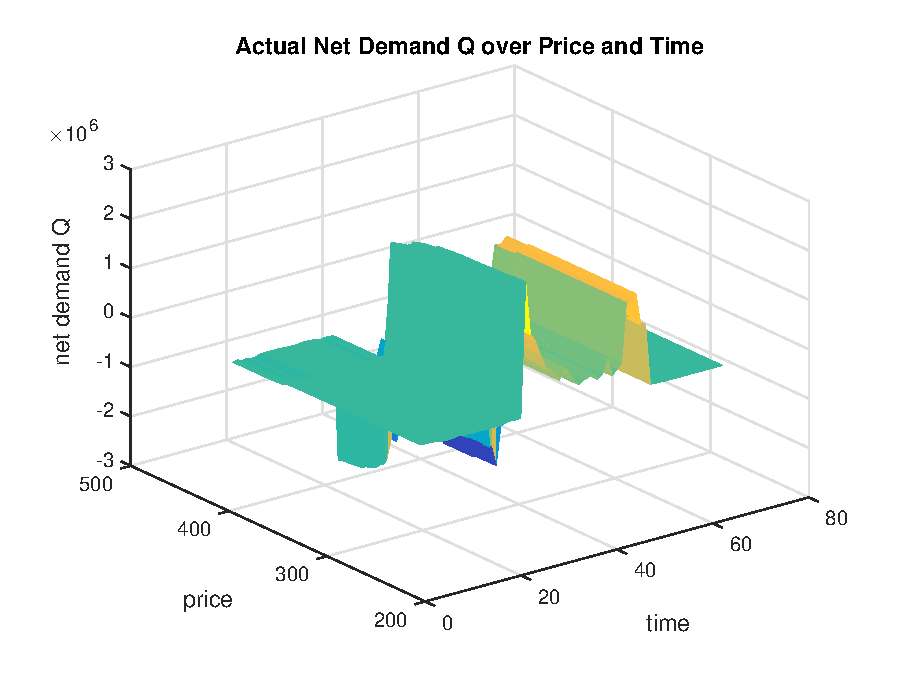
\includegraphics[scale = 0.7]{AAPL_20110401_Calibration_Q.eps}\\
  \caption{The calculated net demand surface $Q$ by price and time, from market data for AAPL as of April 1st, 2011.}\label{fig::AAPL_20110401_Calibration_Q}
\end{figure}
\end{center}

After the net demand surface $\hat{Q}$ is calculated, the net demand sensitivity $\hat{q}$ is calculated by taking the first order difference of $\hat{Q}(p)$, where $p = 0,1,\ldots,S$. That is,

$$
\hat{q}(p,t) = - \frac{\hat{Q}(p, t) - \hat{Q}(p - \Delta p, t)}{\Delta p}
$$
where $p=1,2,\ldots,S$. And $\Delta p = \$1.91$. By this definition, $\hat{q}(p,t)$ is no less than 0, since $\hat{Q}(p, t) \geq \hat{Q}(p - \delta p, t)$ if $\delta p \geq 0$. The discretization of  $q(p,t,\omega ) =\exp{\int_{x=0}^{p}h(x,t,\omega )dx}$ yields

$$
\hat{h}(p,t) = \log(\hat{q}(p,t)) - \log{\hat{q}(p-\Delta p,t)}
$$
where $\delta p$ represents the price partition. The net demand elasticity $\hat{\eta}$ is calculated by

$$
\hat{\eta}(t) = \frac{\hat{Q}(0, t)}{\hat{Q}(0, t) - \hat{Q}(S, t)}
$$
and $0 \leq \hat{\eta}(t) \leq 1$, since $\hat{Q}(0, t) > 0$ and $\hat{Q}(S, t)<0$.

Now we have all the values of $\hat{Q}(p,t)$ with $p = 0,1,\ldots, S$ and $\hat{q}(p,t)$ with $p = 1,2,\ldots, S$ and $\hat{h}(p,t)$ with $p = 2,3,\ldots, S$. Let the $H$ matrix be

$$
H =
\left(
  \begin{array}{ccccc}
    \hat{q}(1,0) & \Delta \hat{h}_{2,0} & \cdots & \Delta \hat{h}_{S,0} & \frac{\Delta \hat{\eta}_{0}}{\sqrt{\hat{\eta}_{0}(1-\hat{\eta}_{0})}} \\
    \vdots & \vdots & \ddots & \vdots & \vdots \\
    \hat{q}(1,T) & \Delta \hat{h}_{2,T} & \cdots & \Delta \hat{h}_{S,T} & \frac{\Delta \hat{\eta}_{T}}{\sqrt{\hat{\eta}_{T}(1-\hat{\eta}_{T})}}  \\
  \end{array}
\right)
$$

We calculate the instantaneous volatilities $\sigma_h$ and $\sigma_{\eta}$ by the method of moments. We use Cholesky and Schur decomposition with respect to calculate $B_{H}=H^{1/2}$, where $b_{\eta,h_p}=0$ except for $b_{\eta,h_S}=1$.

\begin{center}
\begin{figure}
  \centering
  % Requires \usepackage{graphicx}
  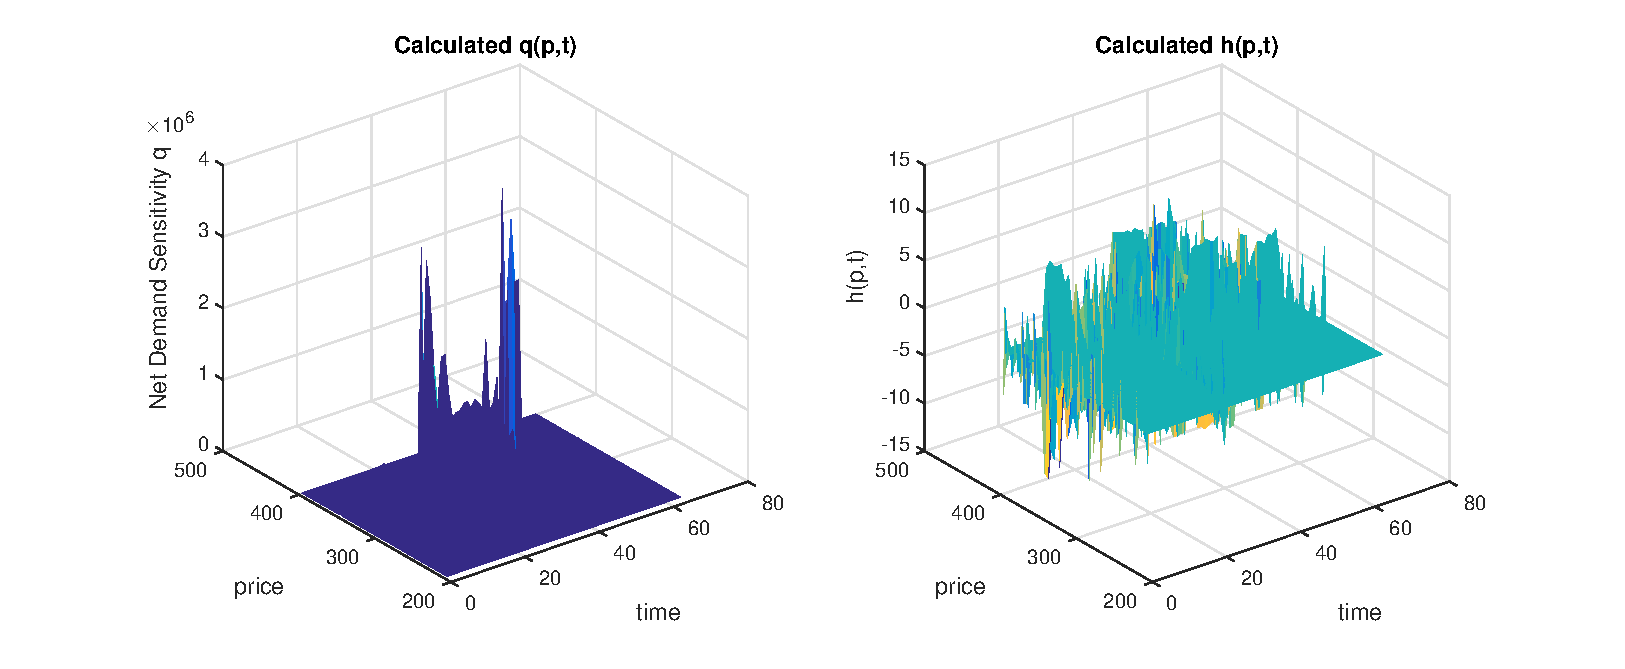
\includegraphics[scale = 0.5]{q_and_h.eps}\\
  \caption{The calculated q(p,t) and h(p,t) from market data for AAPL as of April 1st, 2011.}\label{fig::AAPL_20110401_q_and_h}
\end{figure}
\end{center}


\subsection{Simulation Methodology}
We first simulate the $h(p,t)$ process using the calibrated parameters over simulated time. For simplicity we remove the ''hat'' sign on the parameters. We also assume the $h$ and $q$ processes have zero drift.

\begin{eqnarray*}
\Delta h(p,t) &=& h_p(t+\Delta t) - h_p(t) \\
        &=& \sigma_{h_p} \sum_{i=2}^{S} b_{h_{p, i}} z(i,t) \sqrt{\Delta t \Delta p} \\
        &=& \sigma_{h_p} \sum_{i=2}^{S} b_{h_{p, i}} z(i,t) \sqrt{\Delta t \Delta p} \qquad p = 2, 3, \ldots, S
\end{eqnarray*}

and $h(0,t) = h(1,t) = 0$ for computational convenience. The time step $\Delta t$ is 15 minutes in this case. The boundary condition of the $q(p,t)$ process, $q(1,t)$, is simulated by

$$
q(1,t) = \sigma_{q_0} \sum_{i=2}^{S} b_{q_{0, i}} z(i,t) \sqrt{\Delta t \Delta p}
$$
where $z(i,t)$ is a random normally distributed number. The rest of the numerical $q(p,t)$ values are

$$
q(p,t) = q(1,t) \exp{\sum_{i=2}^{p}h_i(t)} \qquad p = 2, 3, \ldots, S
$$

Then the boundary condition of the net demand $Q(0,t)$ is calculated as

$$
Q(0,t) = \frac{\eta(t)}{2-\eta(t)} \sum_{p=1}^{S} q(p)
$$

which is consistent with the intuition that $Q(0,t) \geq Q(1,t)$ given $q(1,t)\geq 0$. And the rest of the $Q(p,t)$ is

$$
Q(p,t) = [Q(0,t) + \sum_{i=1}^{S}q(i,t)]\eta(t) - [Q(0,t) + \sum_{i=1}^{p}q(i,t)]  \qquad p = 1, 2, \ldots, S
$$
where

\begin{eqnarray*}
\Delta \eta(t) &=& \eta(t+\delta t) - \eta(t) \\
         &=& a_{\eta}(\bar{\eta} - \eta(t)) \Delta t + \sigma_{\eta} \sqrt{\eta(t)(1-\eta(t))}  \sum_{i=2}^{S} b_{\eta,h_p} z(i,t) \sqrt{\Delta t } \\
         &=& a_{\eta}(\bar{\eta} - \eta(t))\Delta t + \sigma_{\eta} \sqrt{\eta(t)(1-\eta(t))} z(S,t) \sqrt{\Delta t }
\end{eqnarray*}

\subsection{Simulation Results on Physical Measure}
The simulated net demand curve under physical measure using the above methods is shown in Figure~\ref{fig::AAPL_20110401_simulated_Q_physical_measure}.

\begin{center}
\begin{figure}
  \centering
  % Requires \usepackage{graphicx}
  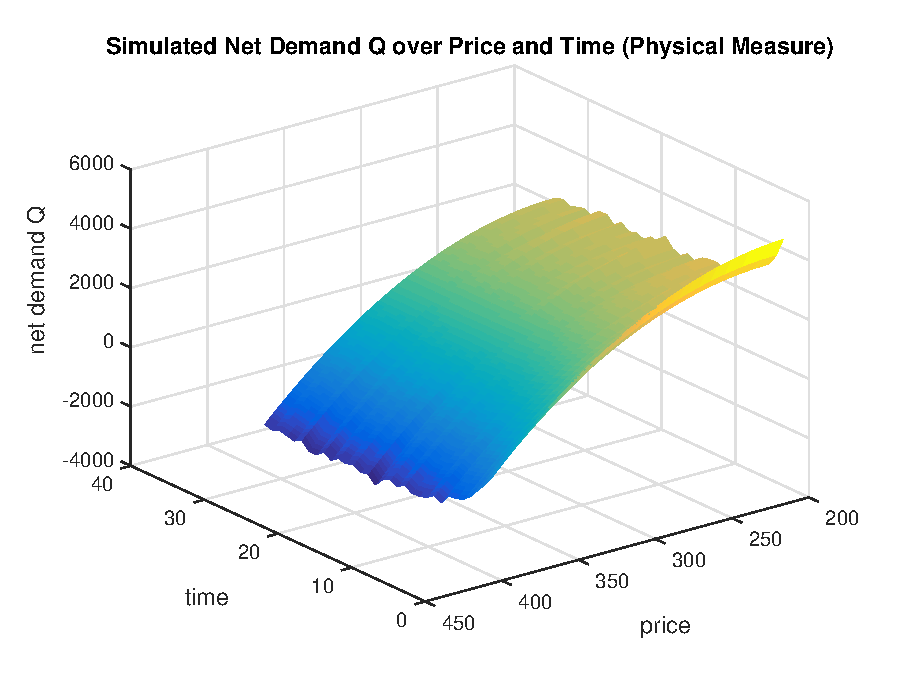
\includegraphics[scale = 0.5]{Simulated_Q_Physical_Measure.eps}\\
  \caption{The simulated net demand surface Q(p,t) under physical measure.}\label{fig::AAPL_20110401_simulated_Q_physical_measure}
\end{figure}
\end{center}

\subsection{Simulation Results on Risk Neutral Measure}
Changing from physical measure simulation to P measure simulate requires the following adjustments on $h(p,t)$ process simulation.

$$
\Delta h(p,t) = \sigma_{h_p} \Sigma_{i=2}^{S} b_{h_{p, i}} [z(i,t) \sqrt{\Delta t \Delta p} - \lambda(i)\sqrt{\Delta p}] \qquad p = 2, 3, \ldots, S
$$

To solve for $\lambda(i)$, let \{$\mu _{Q}$, $a_{Q},\sigma _{Q}$, $b_{Q}\}$ be the parameters of net demand.
Let the volatility of the clearing price be:

\begin{equation*}
\sigma _{\pi }(t,\omega )b_{\pi }(s,t,\omega )=-\frac{\sigma _{Q}(\pi
(t),t)b_{Q}(s,t,\omega )}{q(\pi (t),t,\omega )}
\end{equation*}
\bigskip

Define:

\begin{eqnarray*}
C(\pi ,t) &=&\sigma _{\pi }(t)\sum_{s=0}^{S}\frac{\Delta \lbrack \sigma_{Q}(p,t,\omega )b_{Q}(p,s,t)]}{\Delta p}|_{p=\pi }b_{\pi }(s,t) \\
&=&\sum_{s=0}^{S}\frac{\Delta \lbrack \sigma _{Q}(p,t,\omega )b_{Q}(p,s,t)]}{\Delta p}|_{p=\pi }\sigma _{\pi }(t)b_{\pi }(s,t) \\
&=&-\sum_{s_{2}=0}^{S}\frac{\Delta \lbrack \sigma _{Q}(p,t,\omega)b_{Q}(p,s_{2},t)]}{\Delta p}|_{p=\pi }\frac{\sigma _{Q}(\pi(t),t)\sum_{s=0}^{S}b_{Q}(\pi (t),s,t)}{q(\pi (t),t)} \\
B(\pi ,t) &=&\mu _{Q}(\pi ,t)-\frac{1}{2}\frac{Q(p+1,t) - 2Q(p,t) + Q(p-1,t)}{\Delta p^{2}}|_{p=\pi }+C(\pi ,t) \\
\Sigma (\pi ,s,t) &=&\sigma _{Q}(\pi ,t)b_{Q}(\pi ,s,t)
\end{eqnarray*}
\bigskip

The M.P.R. are, for each $t$ and $\omega $ to find $\lambda (s)$ that
satisfy:%
\begin{equation*}
\sum_{s=0}^{S}\Sigma (\pi ,s)\lambda (s) = B(\pi )
\end{equation*}

The value of $\sigma _{Q}(p,t)b_{Q}(p,s,t)$ is given by ($p > 2$):%
\begin{eqnarray*}
&&\left( Q(0,t)\sigma _{Q_{0}}b_{Q_{0},s}+q(1,t)\sigma _{q_{1}}b_{q_{1},s}+\sum_{y=2}^{S}\exp
(\sum_{i=2}^{y-1}h_{i}(t))\sum_{x=2}^{y-1}\sigma_{h_{x}}b_{h_{x,y}}\right) \eta (t)+ \\
&&\left( [Q(0,t)+\sum_{x=1}^{S}q(x,t)]\sigma _{\eta }\sqrt{\eta (t)(1-\eta
(t))}\right) b_{\eta ,s}+ \\
&&\left( Q(0,t)\sigma_{Q_{0}}b_{Q_{0},s}+q(1,t)\sigma_{q_{1}}b_{q_{1},s}+\sum_{y=2}^{p}\exp
(\sum_{i=2}^{y-1}h_{i}(t))\sum_{x=2}^{y-1}\sigma_{h_{x}}b_{h_{x,y}}\right)
\end{eqnarray*}

The simulated net demand curve under risk neutral measure using the above methods is shown in Figure~\ref{fig::AAPL_20110401_simulated_Q_P_measure}.

\begin{center}
\begin{figure}
  \centering
  % Requires \usepackage{graphicx}
  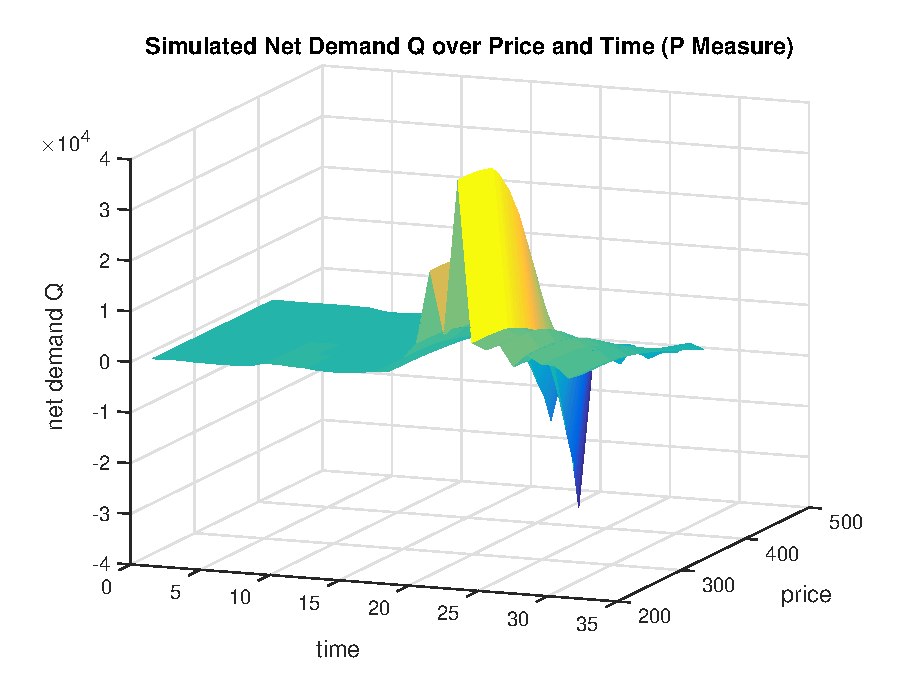
\includegraphics[scale = 0.5]{Simulated_Q_P_Measure.eps}\\
  \caption{The simulated net demand surface Q(p,t) under risk neutral measure.}\label{fig::AAPL_20110401_simulated_Q_P_measure}
\end{figure}
\end{center}

\newpage
\subsection{Option Pricing under Risk Neutral Measure}
With the simulations under risk neutral measure, the corresponding call/put option price, $c(\pi, \omega)$, with strike $K$ at given time $t$ is

\begin{eqnarray*}
c(K) &=& \frac{1}{N} \sum_{\omega} \max\left(\pi(t,\omega)-K,0\right) \\
p(K) &=& \frac{1}{N} \sum_{\omega} \max\left(K - \pi(t,\omega),0\right) \qquad \omega = 1,2,\ldots,N
\end{eqnarray*}

where $\pi$ is the clearing price at simulation time $t$. With the option prices, the implied volatility for different strike levels are calculated by solving

$$
p(K) = BS(\pi,K,r,T,\sigma(K))
$$
where $\pi$ is the clearing price, $K$ is the strike level, $r$ is the interest rate, $T$ is time to maturity and $p$ is the put option price corresponding to the strike $K$.
The implied volatility $\sigma(K)$ is being solved.

The implied volatility smile generated from the equity options at simulation period is shown in Figure~\ref{fig::Put_Option_Vols}.
The implied volatilities by simulations under risk neutral measure are plotted as blue line, which are compared to the real historical implied volatility levels from Bloomberg. The interest rate level is selected as 0.301\%, and the dividend yield is set to 0\%. The maturity of the option is in 10 days. The simulation is evaluated under 500 scenarios.

The at-the-money simulated implied volatility is lined up with the Bloomberg quote, at 25\% level. For low strike options the simulation results tend to underestimate the implied volatility by 5\%~10\%. For high strike options the simulation results tend to overestimate the implied volatility by 5\%~7\%. 

\begin{center}
\begin{figure}
  \centering
  % Requires \usepackage{graphicx}
  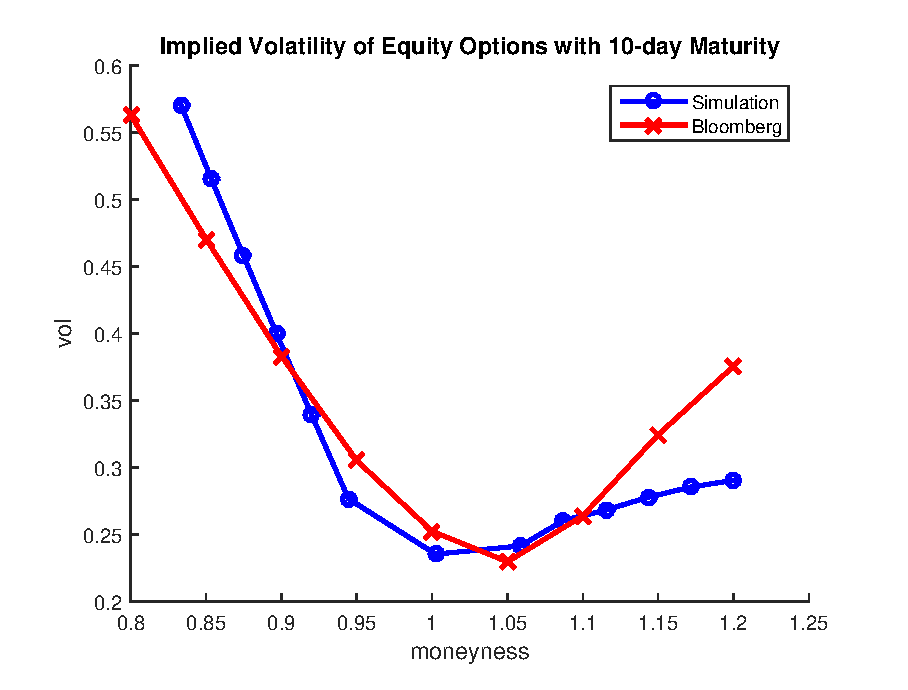
\includegraphics[scale = 0.5]{implied_vol.eps}\\
  \caption{The implied volatility levels from equity options with maturity of 10 days.}\label{fig::Put_Option_Vols}
\end{figure}
\end{center}
\end{document}
